\chapter{The systemic functional theory of grammar} %The systemic functional grammar}
\label{ch:sfg}

Any description of language requires a theory that provides the frame, scope and the necessary concepts. 
%used to describe a grammar i.e. structure, categories, functions, relations and how they relate to one another. 
Having a solid theory of grammar contributes to explaining what language is and how it works. It also frames how language is ought yo be analysed by either human or machines. 
%A grammar, as a description of linguistic rules, is thus framed by a theory of grammar expressing what language is, how it functions and in which ways it shall be describes.

In his seminal paper \citet{Halliday61} addresses the ardent need of the time for a general theory of language and partially answers the proposal for a universal theory of language. He sets out what was known at the time as Scale and Category Grammar. 
In such a model \textit{units} are set up to account for for pieces of language which carry grammatical patterns. They are seen as arranged on a hierarchical \textit{rank} scale of words, groups and clauses. These and other foundational concepts are covered in the first part of this Chapter. 

There are two variants of Systemic Functional Grammars: the \textit{Sydney Grammar} started in 1961 by \citet{Halliday2002} and the \textit{Cardiff Grammar} proposed by \citet{Fawcett2008} which is a simplification and an extension of the Sydney Grammar. To understand the underlying motives and how exactly they are different we shall start looking at the theories of grammar before we look at the grammars proposed in Sydney and Cardiff SFL schools.

This chapter first sets out the basic organisational dimensions of the theory and then discusses comparatively Halliday's \citep{Halliday2002} and Fawcett's \citep{Fawcett2000} SFL.

%Because SFL grammar works with more complex structures than simply word dependencies like Dependency Grammars therefore the pragmatics of this chapter is at large oriented towards describing what constituents and functions can be derived from dependency structure and word classes and what is beyond that of a more semantic nature.

\section{A word on wording}
Before going into deeper discussion I first make terminological clarifications on the terms: grammar, grammatics, syntax, semantics and lexicogrammar. I start with a definitions adopted in ``mainstream'' generative linguistics and then present how the same terms are discussed in systemic functional linguistics.

%Radford1997: A minimalist introiduction to syntax
Radford, a generative linguist, in the ``Minimalist Introduction to Syntax'' (\citeyear{Radford1997}), starts with a description of grammar as a field of study, which, in his words, is traditionally subdivided into two inter-related areas of study: syntax and morphology. %\citep[p.1]{Radford1997}.

\begin{definition}[Morphology (Radford)]\label{def:morphology-min}
Morphology is the study of how words are formed out of smaller units (traditionally called morphemes) \citep[p.1]{Radford1997}.
\end{definition}

\begin{definition}[Syntax (Radford)]\label{def:syntax-min}
Syntax is the study of how words can be combined together to form phrases and sentences. \citep[p.1]{Radford1997}
\end{definition}

%In London school of linguistics this distinction is perceived as unnecessary. %Halliday (on grammar) 2002 
%He take this position to motivate the proposed SFG architecture.
Halliday, in the context of rank scale discussion \citep[p. 51]{Halliday2002}, refers to the traditional meaning of syntax as the \textit{grammar above the word} and to morphology as \textit{grammar below the word}. Such a distinction, he states, has no theoretical status and is deemed as unnecessary distinction. Halliday adopts this position to motivate the architecture of grammar he was developing and is inherited from his precursor, Firth, as he puts it: 
\begin{quote}
	\dots the distinction between morphology and syntax is no longer useful or convenient in descriptive linguistics. \citep[p.14]{Firth1957}
\end{quote}

%[JB] if you say that this is Halliday's position and was used to motivate the architecture of SFG, then no one can complain or disagree, because that is simply a statement of fact.
%[JB] Morphology works with very different principles to syntax (that is why in our versions of many grammar, we have such different realisation rules for morphology and for syntax). 

Radford adds that, traditionally, grammar is not only concerned with the principles governing formation of words, phrases and sentences but also with principles governing their interpretation. Therefore \textit{structural aspects of meaning} are said to be also a part of grammar. 

\begin{definition}[Grammar (Radford)]\label{def:grammar-min}
[Grammar is] the study of the principles which govern the formation and interpretation of words, phrases and sentences. \citep[p.1]{Radford1997}
\end{definition}

Interestingly enough, the Definition \ref{def:grammar-min} makes no mention at all to the lexicon. This is because the formal grammars focus primarily on unit classes and how they are accommodated in various structures and so in formal linguistics the lexicon is often disconnected from the grammar. The systemic grammar, on the other hand, along with formal descriptions of grammatical categories and structures, includes the lexicon as part of grammar to form a \textit{lexicogrammar}. At this point I have to mention that systemic functional grammar is not the only lexicalised one and there are others taking the same approach such as 
%TODO: references needed
Lexical Functional Grammar (LFG), Head Phrase Structure Grammar (HPSG), Combinatory Categorial Grammar (CCG) and others. 

Another important aspect to notice is that the grammar is defined as a field of study rather than a set of rules. De divergence in perspective on the subject led Halliday, since his early papers, to become conscious the difference between a study of a phenomenon with the phenomenon itself. By analogy to language as phenomenon and linguistics as the study of the phenomenon, discussed in  \citep{Halliday1997-linguistics}, Halliday adopts the same wording for \textit{grammar} as phenomenon and \textit{grammatics} as the study of grammar; the same distinction holds for \textit{syntax} and \textit{syntactics}.

\begin{definition}[Grammatics (Halliday)]\label{def:grammatics-halliday}
	Grammatics is a theory for explaining grammar \citep[p.369]{Halliday2002}
\end{definition}

%E. Moravcsik
Moravcsik, another generative linguist, stresses the same distinction, in her ``An introduction to syntax'' \citep{Moravcsik2006}, and presents two ways in which the word \textit{syntax} is used in the literature: (a) in reference to a particular aspect of grammatical structure and (b) in reference to a sub-field of descriptive linguistics that describes this aspect of grammar. 
In her words: 

\begin{quote}
	\dots
	syntax describes the selection and order of words that make well-formed sentences and it does so in as general a manner as possible so as to bring out similarities among different sentences of the same language and different languages and render them explainable. \dots syntax rules also need to account for the relationship between string of word meanings and the entire sentence meaning, on one hand, and relationship between strings of word forms and the entire sentential phonetic form, on the other hand. \citep[p.25]{Moravcsik2006}	
\end{quote}

In her definition of grammar she includes the lexicon and semantics which is a somewhat more explicit statement than Radford's \textit{interpretation}. She is also getting, in Definition \ref{def:grammar-moravcsik}, somewhat closer to what grammar stands for in SFL - Definition \ref{def:grammar-halliday}. 

\begin{definition}[Grammar (Moravcsik)]\label{def:grammar-moravcsik}
... maximally general analytic descriptions, provided by descriptive linguistics, [are] called grammars. A grammar has five components: phonology (or, depending on the medium, its correspondent e.g. morphology), lexicon, syntax and semantics\citep[pp.24--25]{Moravcsik2006}. 
\end{definition}

%Halliday and Matthiessen 1999 - Construing experience through meaning

%Halliday (on grammar) 2002
\begin{definition}[Grammar (Halliday)]\label{def:grammar-halliday}
	To Halliday, lexico-grammar, or for short,simply grammar is a part of language and it means the wording system - the ``lexical-grammatical stratum of natural language as traditionally understood, comprising its syntax, vocabulary together with any morphology the language may display [...]'' \citep[p.369]{Halliday2002}.
\end{definition}

%Another important aspect to note about the generative linguistics is the focus on the formal aspects of language where even the semantics (also referred to as interpretation) refers only to the ``formal aspect of meaning''. 

The last point I want to mention is the approach to semantics. Formal grammars aim to account for the realisation variations, that is formation of words, phrases and sentences along with their arrangements and mention of semantics is often restricted to what may be termed the \textit{formal aspect of meaning}. 

By contrast, a systemic grammar is a functional grammar, which means (among other things) that it is semantically motivated, i.e. ``natural''. 
%TODO: [JB] note that most contemporary theories of grammar assume a close morphism betwene grammar and semantics - this is then also 'natural' (even more generally, this is the long acknowledged operation of iconicity in grammar), so be careful what you state as being about grammar and what is meant to be specific about 'SFG'.
So the fundamental distinctions between formal and functional grammars is the semantic basis for explanations of structure. 
%TODO: [JB] Here you might be better going back to Butler's definitions and distinctions btween formal and functional grammars, as the boundary is by no means clearcut. The way you have it, most modern formal linguists would be alienated: think of CCG, there the relation between semantics and grammar is enforced even more strongly than in SFG: each and every grammar rule is at the same time a semantic rule. This is also in Montague grammar and so is not new. I would phrase these things by placing the basic assumptions of SFG as running alongside these assumptions, not as a distinction that separates SFG from them.

Also, in SFL, the meaning is being approached from a semiotic perspective, placing the linguistic semantics in perspective with the linguistic expression and the real world situation. 
In this respect, \citet{Lemke93} offers a well formulated theoretical foundation that ``human communities are eco-social systems that persist in time through ongoing exchange with their environment; and the same holds true for any of their sub-subsystems [...]'' including language. The social practices constituting such systems are both material and semiotic, with a constant dynamic interplay between the two. \citep[p.387]{Halliday2002}

To Halliday, the term \textit{semiotic} accounts for an orientation towards meaning rather than sign. In other words, the interaction is between \textit{the practice of doing and the practice of meaning}. As the two sets of practices are strongly coupled, Lemke points out that there is a high degree of redundancy between the \textit{material-semiotic interplay}. And it perfectly resonates with Firth's idea of \textit{mutual expectancy} between the text and the situation. This idea of interplay is incorporated in SFL as \textit{language stratification} and is graphically represented in Figure \ref{fig:stratification-sfl}.

\begin{figure}[h]
	\centering
	\begin{tikzpicture}
		\coordinate (o) at (0,0);
		\coordinate (o-11) at (-16em,16em);
		
		\coordinate (A) at (-9,2);
		\coordinate (C) at (-6,6);
		\coordinate (D) at (-1,1);
		
		\draw[thick, name path = mn] (o) arc(315:-360:4em);
		\draw[thick, name path = me](o) arc(315:-360:7em);
		\draw[thick, name path = mx] (o) arc(315:-360:10em);
		
		\draw[thin, white, name path = ref](o)--(o-11);
		
		\path[name intersections={of = ref and mn, name = tgt} ];
		\draw[thick, dashed, name path = plane] ($(tgt-2)!10em!90:(C)$) -- ($(tgt-2)!14em!-90:(C)$);
		\path[name intersections={of = plane and mx, name = tgt2} ];
		
		\draw[thick, <->, postaction={ decorate ,decoration = {text along path, raise=1ex, text align=center,text={Stratification}}}](A) -- +($(D)-(C)$);  % the stratification axis line
		
		\node[align = center] at (-1,1) {Phonology \\ (sounding)};
		\node[align = center] at (-3,3) {Lexicogrammar \\ (wording)};
		\node[align = center] at (-5,5) {Semantics \\ (meaning)};
		
		\node[align = center] at (2,5) {Expression};
		\node[align = center] at (0.4,6.6) {Content};
		
		\coordinate (ec) at (-0.6,2) ;
		
%		\draw[red, fill = red](tgt-1) circle(0.1em);
%		\draw[red, fill = red](tgt-2) circle(0.1em);
%		\draw[red, fill = red](tgt2-1) circle(0.1em);
%		\draw[red, fill = red](tgt2-2) circle(0.1em);
		
		%\fill[yellow, fill opacity=.4] (o) arc(315:393.5:10em) -- (tgt-2) arc (135:300:4em);
		\fill[yellow, fill opacity=.2] (o) arc(315:393.5:10em) -- (tgt2-1) arc (236.5:315:10em);
		
	\end{tikzpicture}
	\caption{The levels of abstraction along the realisation axis}
	\label{fig:stratification-sfl}
\end{figure}
 

Having that said, the stratification axis is a useful dimension to relate the formal and the systemic functional grammars. This is also an instrument employed by Hjelmslev \citep{Taverniers2011}. %TODO: eventually expand here

The SFL model defines language as a resource organised into three strata: phonology (sounding), lexicogrammar (wording) and semantics (meaning). Each is defined according to its level of abstraction on the realisation axis. The realisation axis is divided into two planes: the expression and the content planes. 
Although debate about the precise division continues, for current purpose it is sufficient to see the first stratum (i.e. phonology/morphology) belongs to the \textit{expression plane} and the last two (lexicogrammar and semantics) belong to the \textit{content plane}.
%But the division is not so clear because some parts of semantics and lexicogrammar transcend from content into expression plane. 
In this context, the formal grammar could be localised entirely within the expression plane, including the phonology/morphology, syntax, lexicon while formal semantics, stripped of any explanations in terms of the meaning potential, belongs in the content plane.

\section{Sydney theory of grammar}
\label{sec:sydney-theory-of-grammar}
I start introducing the terms of SFL theory with the Sydney grammar as this is in accordance with the historical development originating with \citet{Halliday2002} defining the categories of the theory fo grammar. He proposes four fundamental categories: \textit{unit}, \textit{structure}, \textit{class} and \textit{system}. Each of these categories is logically derivable from and related to the other ones in a way that they mutually define each other. These categories relate to each other on three scales of abstraction: \textit{rank}, \textit{exponence}, \textit{delicacy}. Halliday also uses three scale types: \textit{hierarchy}, \textit{taxonomy} and \textit{cline}.

\begin{definition}[Hierarchy]\label{def:hierarchy}
	Hierarchy [is] a system of terms related along a single dimension which involves some sort of logical precedence. 
	\citep[p.42]{Halliday2002}. 
\end{definition}

\begin{definition}[Taxonomy]\label{def:taxonomy}
	Taxonomy [is] a type of hierarchy with two characteristics:
	\begin{enumerate}
		\item the relation between terms and the immediately following and preceding one is constant
		\item the degree is significant and is defined by the place in the order of a term relative to following and preceding terms. \citep[p.42]{Halliday2002}
	\end{enumerate}
\end{definition} 

\begin{definition}[Cline]\label{def:cline}
	Cline [is] a hierarchy that instead of being made of a number of discrete terms, is a continuum carrying potentially infinite gradations.
	\citep[p.42]{Halliday2002}. 
\end{definition}

The concept of cline may not necessarily originate in SFL but it is used quite extensively in the domain literature.
Next I define and introduce each category of \textit{grammatics} and the related concepts that constitute the theoretical foundation for the Sydney Theory of grammar.

\subsection{Unit}
\label{sec:unit-sydney}
Language is patterned activity of meaningful organization. The patterned organization of substance (\textit{graphic} or \textit{phonic}) along a linear progression is called \textit{syntagmatic order} (or simply \textit{order}). 

\begin{definition}[Unit]\label{def:unit}
	The unit is a grammatical category that accounts for the stretches that carry grammatical patterns. \citep[p.42]{Halliday2002}.
	The units carry a fundamental \textit{class} distinction and should be fully identifiable in description. \citep[p.45]{Halliday2002}.
\end{definition}

\begin{generalization}[Constituency principles]\label{def:constituency-principles}
	The five principles of constituency in lexicogrammar are:
	\begin{enumerate}
		\item There is a scale or rank in the grammar of every language. That of English (typical of many) can be represented as: clause, group/phrase, word, morpheme.
		\item Each unit consists of \textit{one or more} units of rank next below.
		\item Units of every rank may form complexes.
		\item There is potential for rank shift, whereby a unit of one rank my be downranked to function in a structure of a unit of its own rank or of a rank below. 
		\item Under certain circumstances it is possible for one unit to be enclsoed within another, not as a constituent but simply in such a way as to split the other oe into two discrete parts. \citep[pp.9--10]{Halliday2013} 
	\end{enumerate}
\end{generalization}

The relation between units is that of consistency for witch we say that a unit \textit{consists of} other units. The scale on which the units are ranged is the \textit{rank scale}. The rank scale is a levelling system of units supporting unit composition regulating how units are organised at different granularity levels from clause, to groups/phrases to words and the units of a higher rank scale consist of units of the rank next below. The Table \ref{tab:rank-scale} presents a schematic representation of the rank scale and its derived complexes.

\begin{table}[h]
	\centering
	\begin{tabular}{|l|l|}
		\hline
		{\bf Rank scale $\downarrow$} & {\bf Complexing} \\ \hline
		& Clause complex           \\ \hline
		Clause           &                          \\ \hline
		& Group(/phrase) complex   \\ \hline
		Group(/phrase)   &                          \\ \hline
		& Word complex             \\ \hline
		Word             &                          \\ \hline
		& (Morpheme complex)       \\ \hline
		(Morpheme)       &                          \\ \hline
	\end{tabular}
	\caption{Rank scale of the (English) lexicogrammatical constituency}
	\label{tab:rank-scale}
\end{table}

\begin{generalization}[Rank scale constraints]\label{def:rank-skale-constraints}
	The rank relations are constrained as follows:
	\begin{enumerate}
		\item downward \textit{rankshift} is allowed i.e. the transfer of a given unit to a lower rank.
		\item upward rankshift is not allowed.
		\item only whole units can enter into higher units.\citep[p.44]{Halliday2002}.
	\end{enumerate}
\end{generalization}

The Generalization \ref{def:rank-skale-constraints} taken as a whole means that a unit can include, in what it consists of, a unit of rank higher than or equal to itself but not a unit of rank more than one degree lower than itself; and not in any case a part of any unit. \citep[p.42]{Halliday2002}. 

\subsection{Structure}
%TODO: Top down is good for generation and botton mup for parsing
%TODO: agnation as a clive vs instanciation as a cline | subclassification rel vs class-instance rel
%TODO: Rebekah Wegener PhD SFL thesis online [Parameters of context]: Chapter in SFL theory 

\begin{definition}[Structure]\label{def:structure}
	The structure (of a given unit) is the arrangement of \textit{elements} that take places distinguished by order relationship \citep[p.46]{Halliday2002}. 
\end{definition}

\begin{definition}[Element]\label{def:element}
	The element is defined by the place stated as absolute or relative position in sequence and with the reference to the unit next below \citep[p.47]{Halliday2002}. 
\end{definition}


\begin{figure}[h]
	\begin{tikzpicture}
		\tikzset{
			rect/.style n args={4}{
				draw=none,
				rectangle,
				append after command={
					\pgfextra{%
						\pgfkeysgetvalue{/pgf/outer xsep}{\oxsep}
						\pgfkeysgetvalue{/pgf/outer ysep}{\oysep}
						\def\arg@one{#1}
						\def\arg@two{#2}
						\def\arg@three{#3}
						\def\arg@four{#4}
						\begin{pgfinterruptpath}
						\ifx\\#1\\\else
						\draw[draw,#1] ([xshift=-\oxsep,yshift=+\pgflinewidth]\tikzlastnode.south east) edge ([xshift=-\oxsep,yshift=0\ifx\arg@two\@empty-\pgflinewidth\fi]\tikzlastnode.north east);
						\fi\ifx\\#2\\\else
						\draw[draw,#2] ([xshift=-\pgflinewidth,yshift=-\oysep]\tikzlastnode.north east) edge ([xshift=0\ifx\arg@three\@empty+\pgflinewidth\fi,yshift=-\oysep]\tikzlastnode.north west);
						\fi\ifx\\#3\\\else
						\draw[draw,#3] ([xshift=\oxsep,yshift=0-\pgflinewidth]\tikzlastnode.north west) edge ([xshift=\oxsep,yshift=0\ifx\arg@four\@empty+\pgflinewidth\fi]\tikzlastnode.south west);
						\fi\ifx\\#4\\\else
						\draw[draw,#4] ([xshift=0+\pgflinewidth,yshift=\oysep]\tikzlastnode.south west) edge ([xshift=0\ifx\arg@one\@empty-\pgflinewidth\fi,yshift=\oysep]\tikzlastnode.south east);
						\fi
						\end{pgfinterruptpath}
					}
				}
			}, 
			unit/.style={rect={draw=black, thick}{draw=black, thick}{draw=black, thick}{}},
			place/.style = {rect={draw=black, thick}{}{draw=black, thick}{draw=black, thick}, text width=5.5em,},
			}
		
		\node[unit, text width=\textwidth,align=center](unit-line){};
		\node[above = 0.1em of unit-line](unit-label){Unit};
		%place lines
		{[start chain=l going left,node distance=1em]
			\node[on chain=l,place, below =3em of unit-line](p1){};
			\node[on chain=l,place](p2){};
			\node[on chain=l,place](p3){};
		}
		%place lines to the right
		{[start chain=r going right, node distance=1em,]
			\node[on chain=r,place, right = 1em of p1.east](p4){};
			\node[on chain=r,place](p5){};
			}
		%place labels
		\node[below=0.1em of p1](l3){place_{3}};
		\node[below=0.1em of p2](l2){place_{2}};
		\node[below=0.1em of p3](l1){place_{1}};
		\node[below=0.1em of p4](l4){place_{4}};
		\node[below=0.1em of p5](l5){place_{5}};
		%functional elements
		\node[above = 0.4em of p1, align=center, rectangle, draw, thick,dashed](element1){functional\\element_{3}};
		\node[above = 0.4em of p2, align=center, rectangle, draw, thick,dashed](element2){functional\\element_{2}};
		\node[above = 0.4em of p3, align=center, rectangle, draw, thick,dashed](element3){functional\\element_{1}};
		\node[above = 0.4em of p4, align=center, rectangle, draw, thick,dashed](element4){functional\\element_{4}};
		\node[above = 0.4em of p5, align=center, rectangle, draw, thick,dashed](element5){functional\\element_{5}};
		%order relations
		\draw[bend right,<->,dashed]  (l1) to node [below] {order} (l2);
		\draw[bend right,<->,dashed]  (l2) to node [below] {order} (l3);
		\draw[bend right,<->,dashed]  (l3) to node [below] {order} (l4);
		\draw[bend right,<->,dashed]  (l4) to node [below] {order} (l5);
	\end{tikzpicture}
	\caption{The graphic representation of (unit) structure}
	\label{fig:structure-representation}
\end{figure}

We say that an unit is composed of elements located in places and that its internal structure is accounted via elements in terms of functions and places taken by the lower (constituting) units or lexical items. The graphic representation of the unit structure is depicted in Figure \ref{fig:structure-representation}. The unit structure is referred in linguistic terminology as \textit{constituency} (whose principles are enumerated in Generalization \ref{def:constituency-principles}). In the unit structure, the elements resemble an array of empty slots that are \textit{filled} by other units or lexical items.

\subsection{Class}
\begin{definition}[Class]\label{def:class}
	The class is that grouping of members of a given unit which is defined by operation in the structure of the unit next above \citep[p.49]{Halliday2002}.
\end{definition}

Halliday defines class (Definition \ref{def:class}) as likeness of the same rank ``phenomena'' to occur together in the structure. He adopts a top-down approach stating that the class of a unit is determined by the \textit{function} (Definition \ref{def:function}) it plays in the unit above and not by its internal structure of elements. In SG the structure of each class is well accounted in terms of syntactic variation recognizing six unit classes: \textit{clause}, \textit{prepositional phrase} and \textit{nominal}, \textit{verbal}, \textit{adverbial} and \textit{conjunction} groups.
Sydney grammar is briefly summarised in the Appendix \ref{ch:syntax-overview}. %TODO resolve the appendinx references

\subsection{System}
\label{sec:system}
Structure is a syntagmatic ordering in language capturing regularities and patterns which can be paraphrased as \textit{what goes together with what}. However, language is best represented as a set of system networks (Definition \ref{def:system}) which is a paradigmatic ordering in language describing \textit{what could go instead of what} \citep[p.~22]{Halliday2013}.

This is an essential assumption of systemicists is that the language is best represented in the form of system networks and not as an inventory of structures. The structure of course is a part of language description but it is only a syntagmatic manifestation of the systemic choices \citep[p.23]{Halliday2013}.

\begin{definition}[System]\label{def:system}
	A system is a set of mutually exclusive set of terms referring to meaning potentials in language and are mutually defining. It always means a \textit{closed system} and has the following characteristics:
	\begin{enumerate}
		\item the number of terms is finite,
		\item each term is exclusive of all others,
		\item if a new term is added to the system it changes the meaning of all other terms. \citep[p.41]{Halliday2002}
	\end{enumerate}
\end{definition}

A class is a grouping of items identified by operation in the structure. It is not a list of formal items but an abstraction from them. By increase in \textit{delicacy} the class is broken into secondary classes which stand in the relation of exponent to an element of primary structure of the unit next above. This breakdown gives a system of classes that constitute choices implied by the nature of the class. \citep[p.41]{Halliday2002}

\subsection{Functions and metafunction}
\begin{definition}[Function]\label{def:function}
	The functional categories or functions provide an interpretation of grammatical structure in terms of the overall meaning potential of the language. \citep[p.76]{Halliday2013}.
\end{definition}

Most constituents of the clause structure, however, have more than one function which is called a \textit{conflation of elements}. For example in the sentence ``Bill gave Dolly a rose'', ``Bill'' is the Actor doing the act of giving but also the Subject of the sentence. So we say that Actor and Subject functions are conflated in the constituent ``Bill''. This is exactly the point where the concept of \textit{metafunction} or \textit{strand of meaning} comes into the picture. The Subject function is said to belong to the \textit{interpersonal metafunction} while Actor function belongs in the \textit{experiential metafunction}. 

Halliday identifies three fundamental dimensions of structure in the clause each with distinct meaning: \textit{experiential}, \textit{interpersonal} and \textit{textual}. He refers to them as \textit{metafunctions} and they account of how language meaning has evolved. Table \ref{tab:metafucntions} presents metafunctions and their reflexes in the grammar as proposed in \citep[p.85]{Halliday2013}.

\begin{table}[H]
	\centering
	\begin{tabulary}{\textwidth}{|l|L|L|L|}
		\hline
		{\bf Metafunction} & {\bf Definition(kind of meaning)} & {\bf Corresponding status in clause} & {\bf Favored type of structure}   \\ \hline
		experiential       & construing a model of experience  & clause as representation             & segmental (based on constituency) \\ \hline
		interpresonal      & enacting social relationship      & clause as exchange                   & prosodic                          \\ \hline
		textual            & creating relevance to context     & clause as message                    & culminative                       \\ \hline
		logical            & constructing logical relations    & -                                    & iterative                         \\ \hline
	\end{tabulary}
	\caption{Metafunctions and their reflexes in the grammar}
	\label{tab:metafucntions}
\end{table}

\begin{generalization}[Exhaustiveness principle]\label{def:exhaustiveness}
	Everything in the wording has some function at every rank but not everything has a function in every dimension of structure. \citep{Halliday2002,Halliday2013}
\end{generalization}

With respect to structure and metafunctions, Halliday formulates the general principle of \textit{exhaustiveness} (Generalization \ref{def:exhaustiveness}) saying that clause constituents have at least one and may have multiple functions in different strands of meaning, however it does not mean that it must have a function in each of them. 

This principle implicitly relates to the economic property of language meaning that it naturally evolves towards the shortest and most effective way of expressing a meaning. There is nothing meaningless thus every piece of language must be explained and accounted for in the lexicogrammar. 

\subsection{Lexis and lexicogrammar}
In SFL the terms \textit{word} and \textit{lexical item} are not really synonymous. They are strongly related but they refer to different things. The term ``word'' is reserved (in early Halliday) for the grammatical unit of the lowest rank whose \textit{exponents} are lexical items. %While word refers to the unit of structure below the group/phrase rank and above the morphemes, the lexical item is defies as follows. 

\begin{definition}[Lexical Item]\label{def:lexical-item}
	In English, a lexical item may be a \textit{morpheme}, \textit{word} (in traditional sense) or \textit{group (of words)} and it is assigned to no rank. \citep[p.60]{Halliday2002}
\end{definition}

Examples of lexical items are all of the following ones: `` 's '' (the possessive morpheme), ``house, walk, on'' (words in traditional sense) and ``in front of, according to, ask around, add up to, break down'' (multi word prepositions and phrasal verbs)

If most linguists treat the grammar and lexis as discrete phenomena, Halliday brings them together as opposite poles of the same cline. We say that they are paradigmatically related through delicacy relation. He refers to this merge as \textit{lexicogrammar} and he expressed his dream that one day linguists will be able to turn whole linguistic form into (lexico)grammar showing that lexis is the most delicate grammar. 

\citet{Hasan2014}, explores the reality of Halliday's dream in terms of project feasibility and exploring the implications of what would it mean to turn the ``whole linguistic form into grammar''. This then implies two completely new assumptions: that lexis is not form and that its relation to semantics is unique (challenging the problems of polysemy). It would be the function of the lexicogrammar to map the multiple \textit{meta-functional strata} into a unified structure. 


%%%%%%%%%%%%%%%%%%%%%%%%%%%%%%%%%%%%%%%%%%%%%%%%%%%%%%%%%%%%%%%%%
\section{Cardiff Theory of grammar}
\label{sec:cardiff-theory-grammar}
This section present the theory of grammar as conceived by Robin Fawcett at University of Cardiff. The biggest difference to Hallidayan theory is renouncing the concept of rank scale which has an impact on the whole theory. As a consequence, to accommodate the lack of rank-scale, Fawcett adapts the definitions of the fundamental concepts and slightly changes the choice of words.

In \citeyear{Fawcett2000}, Robin Fawcett presents a theory of grammar in contrast to some aspects of Michael Halliday's grammar \citeyear{Halliday2002}. One of the main differences is the rejection of the rank scale concept. Another is the bottom-up approach to unit definition as opposed to top-down one advocated by Halliday. These two and few other discrepancies have quite an important implication on the overall theory of grammar and of course the grammar itself. 

\citet{Fawcett2000} proposes three fundamental categories in the theory of grammar: \textit{class of unit}, \textit{element of structure} and \textit{item}. Constituency is a relation accounting for prominent compositional dimension of language. However a unit does not function directly as a constituent of another unit but via a specialised relation. Fawcett breaks down constituency into three relations: \textit{componence}, \textit{filling} and \textit{exponence}. Informally is said that a unit is composed of elements which are either filled by another unit or expounded by an item. He also proposes three secondary relations of \textit{coordination}, \textit{embedding} and \textit{reiteration} to account for the full range of syntactic phenomena.

\subsection{Class of units}
\begin{definition}[Class of Unit]\label{def:class2}
	The class of unit [...] expresses a specific array of meanings that are associated with each one of the major classes of entities in semantics [...and] are to be identified by the elements of their internal structure \citep[p.195]{Fawcett2000}. 
\end{definition}

Class of unit is determined based on its internal structure i.e. by its elements of structure (and not by the function it plays in the parent unit).

Fawcett takes a semantic stance in classifying units which in line with Saussurean approach to language. He proposes that in English there are four major semantic classes of entities: situations, things, qualities (of situations and things) and quantities (typically of things but also of situations and qualities) corresponding to major syntactic units of \textit{clause}, \textit{nominal group}, \textit{prepositional group}, \textit{quality group} and \textit{quantity group} \citep[p.~193--194]{Fawcett2000} along with a set of minor classes such as \textit{genitive cluster } and \textit{proper name cluster}. 

His classification is based on the idea that the syntactic and semantic units are mutually determined and supported by grammatical patterns. However those patterns are beyond the syntactic variations of the grammar and blend into lexical semantics.

\subsection{Element of Structure}
\label{sec:elements-of-structure}
\begin{definition}[Element of Structure]\label{def:elementStructure}
	The elements of structure are immediate components of classes of units and are defined in terms of their \textit{function} in expressing meaning and not in terms of their absolute or relative position in the unit. \citep[pp.213--214]{Fawcett2000}. 
\end{definition}

\begin{generalization}[]
	Definition \ref{def:elementStructure} leads to the following two principles:
	\begin{enumerate}
		\item Every element in a given class of unit serves a function in that unit different from the function of the sibling elements.
		\item Every element in every class of unit will be different from every element in every other class of unit. \citep[p.214]{Fawcett2000}
	\end{enumerate}
\end{generalization} 

The elements (of structure) are functional slots which define the internal structure of an unit but still they are \textit{located} in \textit{places}. One more category that intervenes between element and unit is the concept of \textit{place} which become essential for the generative versions of grammar.

There are two ways to approach place definition. The first, is to treat places a positions of elements relative to each other (usually previous). This leads to the need of an \textit{anchor} or a  \textit{pivotal element} which may not always be present/realised. 

The second, is to treat places as a linear sequence of locations at which elements may be located, identified by numbers ``place 1'', ``place 2'' etc. This place assignment approach is absolute within the unit structure and makes elements independent of each other. This approach has been used in COMMUNAL and Penman projects. 

\subsection{Item}
\begin{definition}[Item]\label{def:item}
	The item is a lexical manifestation of meaning outside syntax corresponding to both words (in the traditional sense), morphemes and either intonation or punctuation (depending whether the text is spoken or written). \citep[pp.226--232]{Fawcett2000}. 
\end{definition}

Items correspond to the leaves of syntactic trees and constitute the raw \textit{phonetic} or \textit{graphic} manifestation of language. The collection of items of a language is generally referred as \textit{lexis}.

Since items and units are of different nature, the relationship between an element and a (lexical) item must be different from that to a unit. We say that items \textit{expound} elements and not that they \textit{fill} elements as units do.  

In traditional grammar \textit{word classes} or \textit{parts of speech} are a commonly accepted concept. However in SFL, it plays rather an orientation or an approximation role, precisely because the word classes do not properly correspond to the elements they expound. So terms as \textit{noun} or \textit{adjective} are useful to denote a class of words that expound a certain element of the structure, but such word class to element correspondence shall by no means treated as definite rule.

\subsection{Componence}
\label{sec:componence}
\begin{definition}[Componence]\label{def:componence}
    Componence is the part-whole relationship between a unit and the elements it is composed of. \citep[p.244]{Fawcett2000}. 
\end{definition}

Note that componence is not a relationship between a unit and its places, the latter, as discussed in Section \ref{sec:elements-of-structure}, simply locationally relate elements of a unit to each other. 

Componence intuitively implies a part-whole constituency relationship between the unit and its elements. But this is not the only view. Another perspective is the concept of \textit{dependency} or strictly speaking \textit{sister or sibling dependency} (because the traditional concept of dependency is parent-daughter relation). However the sister dependency is not necessary in the grammar model and is a by-product or second order concept that can be deduced from the constituency structure. 

The (supposed) dependency relation between a modifier and the head, in the framework of SFG is, not a direct one that form-centered linguists consider to be. They simply assume that what modifier modifies is the head. Here however the general function of the modifiers is to contribute to the meaning of the whole unit which is anchored by the head. For example, in the nominal group, the modifier contributes to the description of the referent stated by the head. So the head realises one type of meaning that relates the referent while modifier realises another one. Both of them describe the referent via different kinds of meaning, therefore they are related indirectly to each other because the modifier does not modify the head but the referent denoted by the head. \citep[p.216]{Fawcett2000}

Moreover the dependency relations are expressed between system networks and according to Fawcett this is the true place for dependencies in SFL. 

\subsection{Filling and the role of probabilities}
\begin{definition}[Filling]\label{def:filling}
    Filling is the probabilistic relationship between a element and the unit lower in the tree that operates at that element. \citep[p.238, 251]{Fawcett2000}. 
\end{definition}

Fawcett renounces the concept of rank scale and alternatively proposed the concept of \textit{filling probabilities}. The probabilistic predictions are made in terms of filling relationship between a unit and an element of structure in a higher unit in the tree rather than being a relationship between units of different ranks. This places focus from the fact that a unit is for example a group, to what group class it is. 

In this line of though, some elements of a clause are frequently filled by groups, but some other element almost never being rather expounded by items. The frequency varies greatly and is an important factor for predicting or recognizing either the unit class or the element type in the filling relationship. 

Filling may add a single unit to the element of structure or it can introduce multiple coordinated units. Filling also makes possible the embedding relation. Both, coordination and embedding relations makes it possible to deal without inter-clausal \textit{hypotaxis} and \textit{parataxis} relations described in Sydney Grammar.

Note also that filling and componence are two complementary relations that occur in the syntactic tree down to the level when the analysis moves out of abstract syntactic categories to more concrete category of items via the relationship of exponence. 

\subsection{A few more concepts}
\begin{definition}[Exponence]\label{def:exponence}
	Exponence is the relation by which an element of structure is realised by a (lexical) item \citep[p.254]{Fawcett2000}. 
\end{definition}

%\subsection{coordination}
\begin{definition}[Coordination]\label{def:coordination}
	Coordination is the relation between units that fill the same element of structure \citep[p.263]{Fawcett2000}. 
\end{definition}

Coordination is usually marked by an overt \textit{Linker} such as \textit{and}, \textit{or}, \textit{but}, etc. and sometimes it is enforced by another linker that introduces the first unit such as \textit{both}. 

Coordination is through by Fawcett as being not between syntactic units but between mental referents. It always introduces more than one unit which are syntactically and semantically in similar (somehow) resulting in a \textit{syntactic parallelism} which often leads to \textit{ellipsis}.

%\subsection{Reiteration}
\begin{definition}[Reiteration]\label{def:reiteration}
	Reiteration is the relation between successive occurrences of the same item expounding the same element of structure  \citep[p.271]{Fawcett2000}. 
\end{definition}

Reiteration often is used to create the effect of emphasis such as for example ``she's very very nice!''. Like coordination, reiteration is a relation between entities that fill the same element of the unit structure which is problematic in my opinion and I further discuss it in Section \ref{sec:coordination}.

%\subsection{Embedding}
\begin{definition}[Embedding]\label{def:embedding}
	Embedding is the relation that occurs when a unit fills an element of the same class of units, i.e. when a unit of the same class occurs (immediately) above it in the tree structure \citep[p.264]{Fawcett2000}. 
\end{definition}

Fawcett opens embedding as a general principle as opposed to exceptional/controlled embedding indicated by Halliday. I will further discuss it in the context of rank-scale concept in Section \ref{sec:rank-system}

%\subsection{Conflation}
\begin{definition}[Conflation]\label{def:conflation}
	Conflation is the relationship between two elements that are filled by the same unit having the meaning of ``immediately after and fused with'' and function as one element\ \citep[pp.249--250]{Fawcett2000}. 
\end{definition}

Conflation is useful in expressing multi-faceted nature of language when for example syntactic and semantic elements/functions are realised by the same unit for example the Subject and the Agent or Complement and Affected. Also conflation relations frequently occur between syntactic elements as well such as for example the Main Verb and Operator or Operator and Auxiliary Verb.

\begin{definition}[Taxis]\label{def:taxis}
	\textit{Taxis} represents the degree of interdependency between units systematically arranged in a linear sequence where \textit{parataxis} means equal and \textit{hypotaxis} means unequal status of units forming a \textit{nexus} together.
\end{definition}

\begin{figure}[!ht]
	\centering
	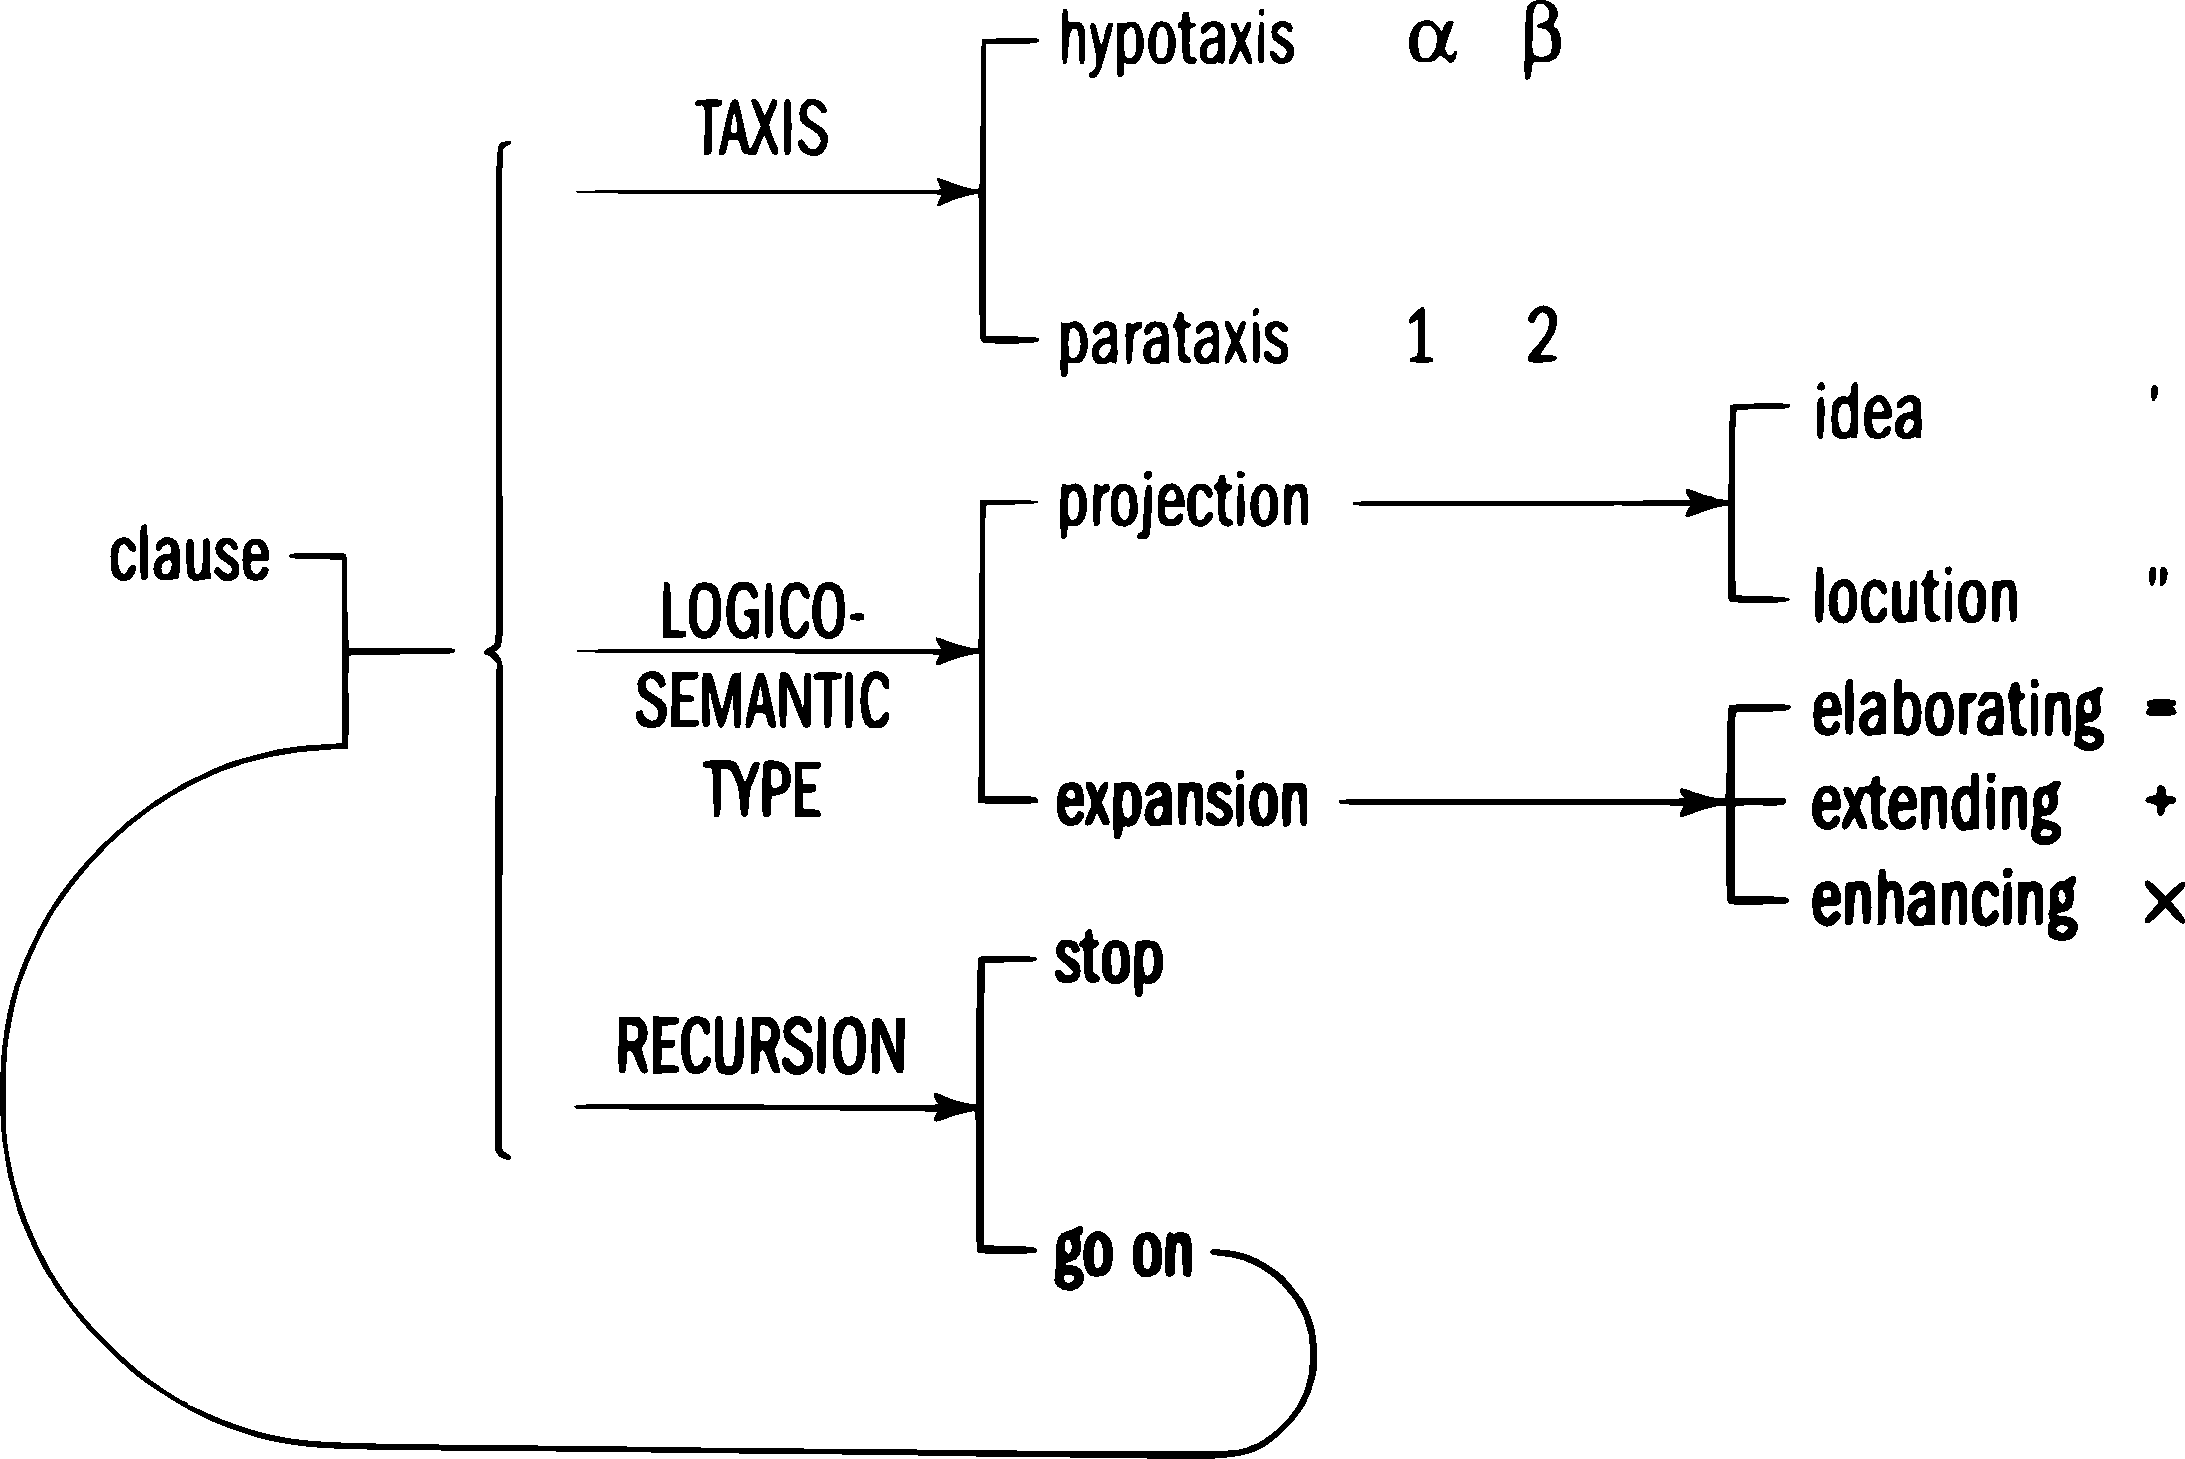
\includegraphics[width=0.678\linewidth]{Figures/SFL-grammar/taxis.pdf}
	\caption{Types of relations between clauses \citep[p.438]{Halliday2013}}
	\label{fig:taxis}
\end{figure}

Taxis play a central role in explaining the textual cohesion. Figure \ref{fig:taxis} depicts the Taxis and clause logico-semantic relations in a single system network. Here taxis relations are employed in explaining how clauses form a nexus with certain tactic relations to one another \citep[pp. 438 -- 443]{Halliday2013}. These concepts nevertheless are very useful at describing unit relations not only at the group and clause ranks but all the way down to smallest linguistic unit such as morphemes and phonemes. I will also employ the concept of taxis in the discussion of dependency relations in Section \ref{sec:cross-theoretical-bridge}. Next I discuss the strengths and weaknesses of the two schools with a pragmatic goal of parsing in mind. 

%\section{Critical discussion on the categories of the theory of grammar: a conciliation of the two theories}
\section{Critical discussion on both theories}

The two sections above cover the definitions and fundamental concepts from each of the two systemic functional theories of grammar. Current work uses a mix of concepts from both theories and this section discusses in detail what and why is being adopted attempting a rather pragmatic reconciliation than a theoretical debate. Next I draw parallels and highlight correspondences between Sydney and Cardiff theories of grammar and where needed alter and present my position on the matter. 

\subsection{Relaxing the rank scale}
\label{sec:rank-system}
%TODO: it is problemantic the fact that when switching metafunction we get a switch in the rank scale for a primary unit of analisys
%TODO: diconnect syntax and metafunctions.
%TODO: metafunctional dimesion breaks down when we look at the context

The \textit{rank scale} proposed by \citet{Halliday2002} became overtime a highly controversial concept in linguistics. Whether it is a suitable for grammatical description or not still continues up to date. The historic development of this polemic is documented in \cite[p.309--338]{Fawcett2000}. %Some strong opponents of the rank scale are Hudson, Huddleston and Fawcett.

%The hierarchy of scale varies across languages and for English there are only three levels: clause, group and word. At each rank level of the scale each unit shall be unambiguously described so that it can be identified and distinguished from others. This is the \textit{``total accountability''} principle seems attainable from the descriptive perspective however is quite difficult to fulfil in generative terms.

I consider rank scale a very useful dimension for unit classification and placement but the definition laid by the Sydney school is too rigid and thus I propose to relax it into a weaker version of it. The relaxation consists of dropping completely the \textit{rank scale constraints} as enunciated in Generalization \ref{def:rank-skale-constraints}. An immediate consequence is that the \textit{embedding} relation can be broadly defined as a naturally occurring phenomena in language at all ranks and not only for clauses as initially proposed.

% The three principles of the rank scale: 
%\begin{enumerate}
%	\item[(a)] that the units of a higher rank can be rank-shifted downwards,
%	\item[(b)] upwards rank-shift is not possible and
%	\item[(c)] only whole units can enter into higher units 
%\end{enumerate}

Halliday's theory allows the downwards rank shift, forbids upwards rank shift and restricts the composition relation to engage only with whole units. Thus the unit may be composed of units of equal rank or a rank higher and cannot be composed of units that are more than one rank lower or parts of other units. The consequence of above is that each element of the clause is filled by a group which has its elements expounded by words. 
\begin{exe}
	\ex \label{ex:small-wooden} some very small wooden ones
\end{exe}

The above rules often pose analysis difficulties and complications. For example in nominal groups what seems to be an element is not a single word but a group of words. Consider example \ref{ex:small-wooden} where Epithet \textit{``very small''} is not a single word but a group \citep[pp.~390--396]{Halliday2013}. This kind of phenomena introduced a \textit{substructure} of modifiers and heads (see analysis in table \ref{tab:example-substructure-analisys}) which complicates the general structure of the nominal group. Accordingly, the Epithet \textit{``very small''} is composed of a head ``small'' and a modifier ``very''. This kind of intricate cases can be simplified through rank-shift constraints allowing the elements of a group to be filled by other groups or expounded by words. 

\begin{table}[H]
	\centering
	\begin{tabular}{|c|c|c|c|c|}
		\hline
		\textbf{some} & \textbf{very} & \textbf{small} & \textbf{wooden} & \textbf{ones} \\ \hline
		\textit{Deictic} & \multicolumn{2}{c|}{\textit{Epithet}} & \textit{Classifier} & \textit{Thing} \\ \hline
		\multicolumn{4}{|c|}{\textit{Modifier}} & \textit{Head} \\ \hline
		\textit{} & \textit{Sub-Modifier} & \textit{Sub-Head} & \textit{} & \textit{} \\ \hline
	\end{tabular}
	\caption{Sydney analysis of Example \ref{ex:small-wooden}}
	\label{tab:example-substructure-analisys}
\end{table}

%
An approach to describe units outside the rank-scale was suggested by \cite{Fawcett2000} and \cite{Butler1985}. Because units are carriers of a grammatical pattern, they can be described in terms of their internal structure instead of their potential for operation in the unit above.

Fawcett proposes complete abandonment of rank scale replaces it with the filling probabilities to guide the unit composition simply mapping elements to a set of legal unit classes that may fill it. The above example, in CG the \textit{``very small''} is analysed as a quality group that plays the role of Modifier (CG) in the nominal group as in table \ref{tab:example-substructure-analisys-cardiff}.

\begin{table}[H]
	\centering
	\begin{tabular}{|c|c|c|c|c|}
		\hline
		\textbf{some} & \textbf{very} & \textbf{small} & \textbf{wooden} & \textbf{ones} \\ \hline
		\textit{Quantifying Determiner} & \multicolumn{2}{c|}{\textit{Modifier}} & \textit{Modifier} & \textit{Head} \\ \hline
		\multirow{2}{*}{\textit{}} & \multicolumn{2}{c|}{\textit{Quality Group}} & \multicolumn{2}{c|}{\multirow{2}{*}{\textit{}}} \\ \cline{2-3}
		& \textit{Degree Tamperer} & \textit{Apex} & \multicolumn{2}{c|}{} \\ \hline
	\end{tabular}
	\caption{Cardiff analysis of Example \ref{ex:small-wooden}}
	\label{tab:example-substructure-analisys-cardiff}
\end{table}

I maintain the idea of ranking the syntactic units because it is a pertinent classification with a clear correspondence to the types of meaning structures in the ideational space.

However I drop the constituency constraints and hence allowing the flexibility for elements to be filled by other units or in other words allow unit embedding. This approach removes the need of sub-structures in the unit elements reducing thus the structural complexity.

The rank system constrains had consequences on the phenomena of embedding defined by Halliday in Definition \ref{def:embedding0}, which I consider way too restrictive.

\begin{definition}[Embedding (strict)]\label{def:embedding0}
	Embedding is the mechanism whereby a clause or phrase comes to function as a constituent within the structure of a group, which is itself a constituent of a clause. \citep[p.242]{Halliday2013}
\end{definition}

The weakening of constituency constrains makes embedding a normal (as defined in broad sense \ref{def:embedding} by Fawcett) rather than an exceptional (as defined in a strict sense in \ref{def:embedding0} by Hallliday) phenomena. And I agree with Fawcett's definition because the human language allows construction of units that contain other units within them regardless of their class.

\subsection{The unit classes}
Fawcett drops the concept of rank system (discussed in Section \ref{sec:rank-system}) and through a bottom-up approach redefining the class as a ``class of unit'' as in \ref{def:class2}.

He adopts Saussurean perspective on language which states that semantics and syntax are strongly intertwined with each other so major semantic classes of entities correspond to the major syntactic units. This lead Fawcett to take a semantic basis for classifying syntactic units into: clause, nominal group, prepositional group, quality group and quantity group \citep[p.~193--194]{Fawcett2000} along with a set of minor classes such as genitive and proper name clusters. 

The problem with this approach is that these classes are beyond the syntactic variations of the grammar and blend into lexical semantics which makes it difficult to apply to parsing, at least nowadays with current state of word classification.   

In the current project I turn to Sydney classification of syntactic units that is close in line with traditional syntactic classification \citep{Quirk1985}. I adopt the clause as a unit plus the four group classes of Sidney grammar depicted in Figure \ref{fig:group-classes}.

\begin{figure}[H]
	\centering
	\begin{subfigure}{.5\textwidth}
		\centering
		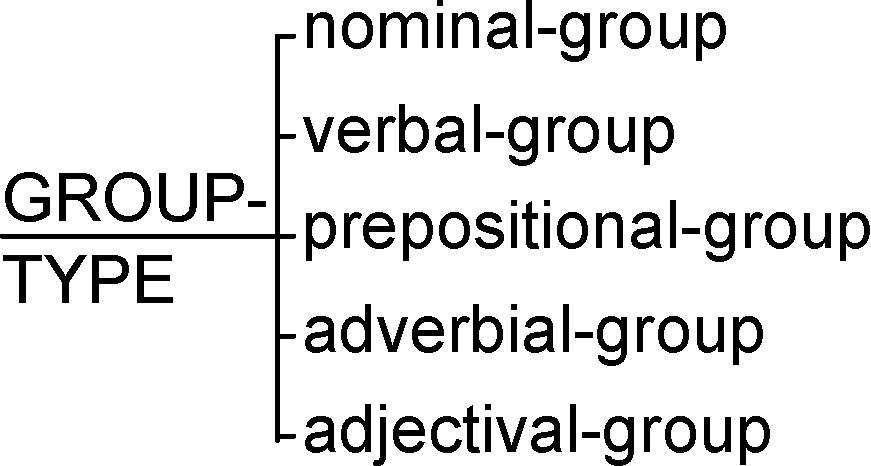
\includegraphics[width=0.57\linewidth]{Figures/SFL-grammar/group-classes.pdf}
		\caption{The group classes}
		\label{fig:group-classes-sub1}
	\end{subfigure}%
	\begin{subfigure}{.5\textwidth}
		\centering
		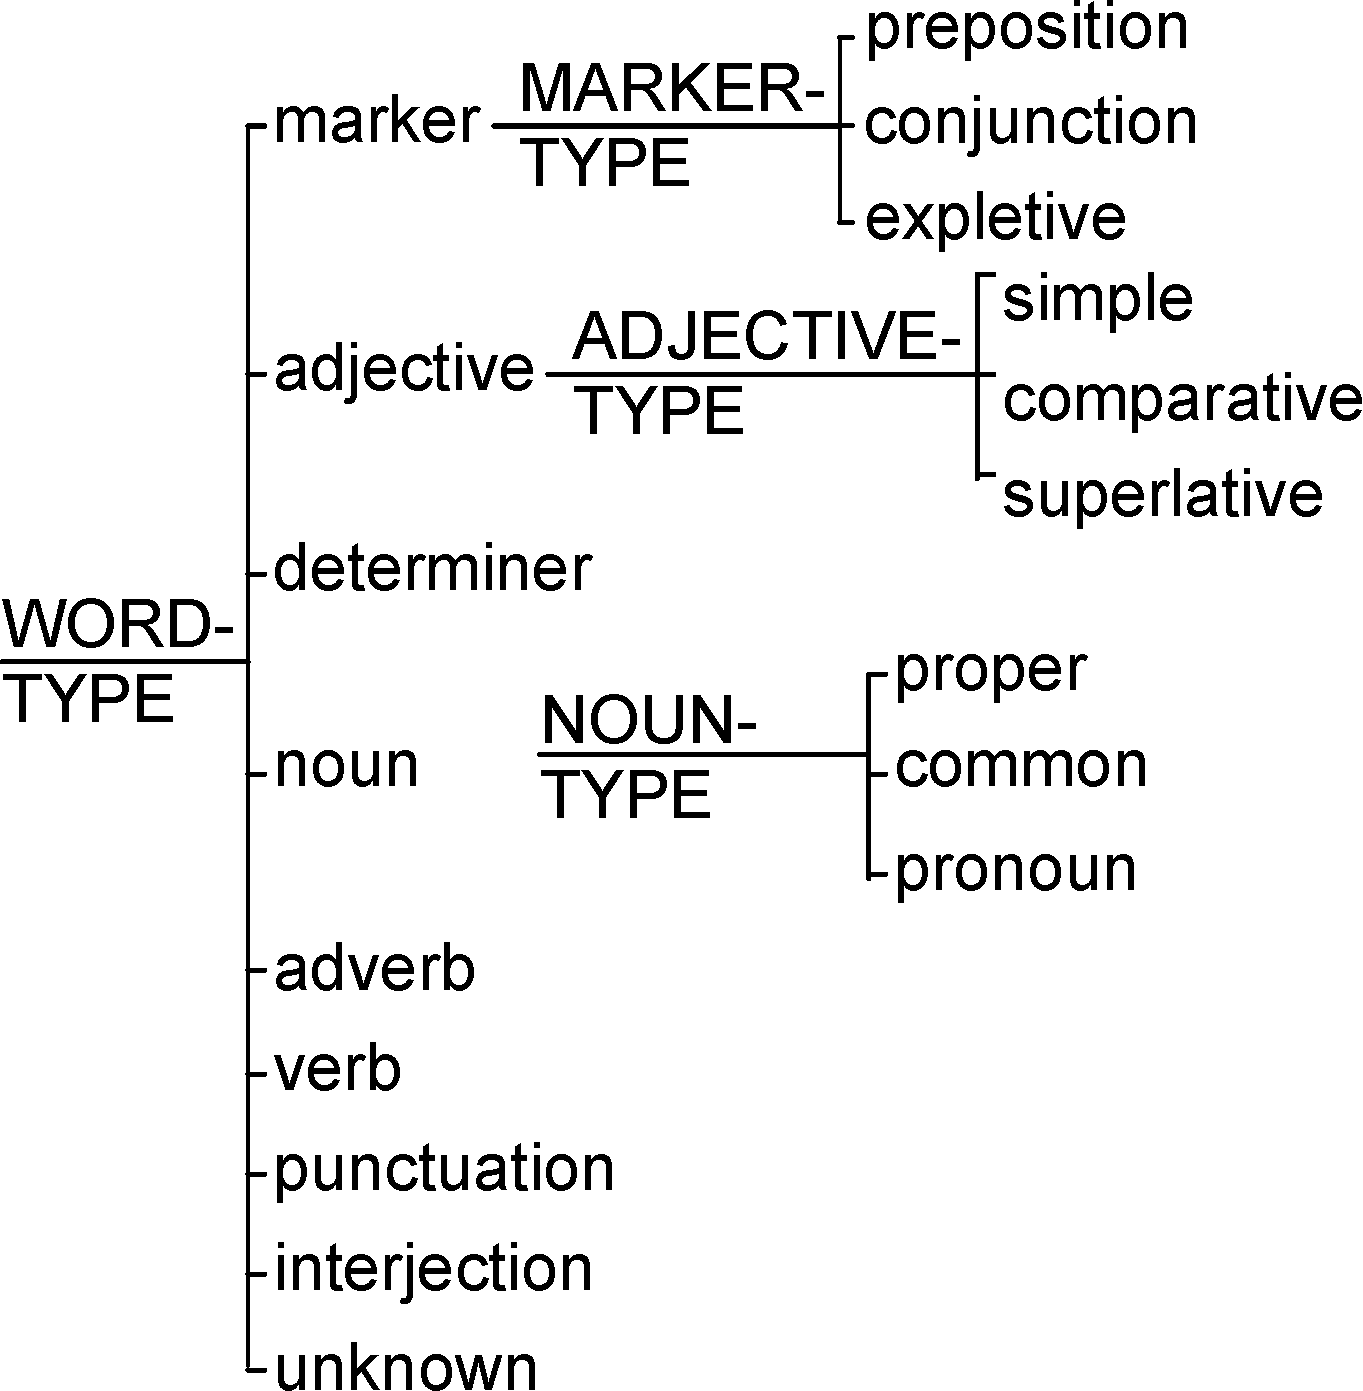
\includegraphics[width=0.9\linewidth]{Figures/SFL-grammar/word-classes.pdf}
		\caption{The word classes}
		\label{fig:group-classes-sub2}
	\end{subfigure}
	\caption{The group and word classes}
	\label{fig:group-classes}
\end{figure}

\subsection{The structure}
The \textit{unit} and \textit{structure} are two out of the four fundamental categories in the systemic theories of grammar. Sydney and Cardiff theories vary in their perspectives on \textit{unit} and \textit{structure} influencing how units are defined and identified.

For Halliday, the \textit{structure} (Definition \ref{def:structure}) characterises each unit as a carrier of a pattern of a particular order of \textit{elements}. The order is not necessarily linear realisation sequence but a theoretical relation of relative or absolute placement. This perspective has been proved useful in generation exercises where unit placement evolves in the realisation process.

The Cardiff School take a bottom up approach and defines class in terms of its internal structure describing a relative or absolute order of elements. This sort of syntagmatic account is precisely what is deemed useful in parsing and is the one adopted in this thesis. It is well established algorithmically how to recognise classes and construct them bottom up. So in our case easier to let the unit class emerge from recognition of constituent part-of-speech (word classes) and dependency relations between words or sequence of lower unit classes. In other words the unit class is defined by the unit structure and not by it's function in the parent unit, as Sydney school predicates, and this is precisely the reason why creation of constituency structure is computationally accessible. 


\subsection{Syntactic and semantic Heads}
%TODO: should this discussion of semantic and syntactic heads be here?
%TODO: provide Hallidayan analysis, my analisys and Cardiff analysis
%\todo{Should this discussion of semantic and syntactic heads be moved somewhere else?}
In SFG the heads may be semantic or syntactic. In most cases they coincide but there are exceptions when they differ or even miss. This is especially an important topic in the discussions of the nominal group structure on which \citet{Halliday2013} offer a thorough examination but \citet{Fawcett2000} offers us a more generic perspective on this issue.

Consider the example of nominal group ``a cup of tea'' analysed in three different ways in the Table \ref{tab:the-head-differences}. The Sydney Grammar offers two analyses in which the semantic and the syntactic heads differ. In the \textit{experiential} analysis the head is ``tea'' which functions as \textit{Thing}, while in the \textit{interpersonal} analysis the head is ``cup'' which functions as \textit{Head}. 

Cardiff Grammar does not make the Head/Thing distinction because the functional elements are already established based on semantic criteria.  discussed in subsection \ref{sec:nominal-group}. Nevertheless the logical analysis of SG resonates closely with the traditional ``semantically blinded'' grammars because it always provides a syntactic Head even if differs from the ``pivotal element'' of the group.

\begin{table}[h]
	\centering
	\begin{tabular}{|c|c|c|c|c|c|}
		\hline
		\multicolumn{2}{|c|}{} & \textbf{a} & \textbf{cup} & \textbf{of} & \textbf{tea} \\ \hline
		\multirow{2}{*}{Sidney Grammar} & experiential & \multicolumn{3}{c|}{\textit{Numerative}} & \textit{Thing} \\ \cline{2-6} 
		& interpersonal & \textit{Modifier} & \textit{Head} & \multicolumn{2}{c|}{\textit{Qualifier}} \\ \hline
		\multicolumn{2}{|l|}{Cardiff Grammar} & \multicolumn{2}{c|}{\textit{Quantifying Determiner}} & \textit{Selector} & \textit{Head} \\ \hline
	\end{tabular}
	\caption{Example of dispersed semantic and syntactic heads}
	\label{tab:the-head-differences}
\end{table}

Fawcett argues that none of the constituting elements of the unit is mandatory realised even the so called \textit{``pivotal element''} which is the group defining element. The logical structure heads are always realised and correspond dependency relations established in the DG. Depending on the unit class logical structure heads are conflated with specific functions, for instance in nominal group the Head is usually conflated with the Thing, in quality group with the Apex, in quantity group with the Amount, in clause with the Main Verb and so on. But in language it is not unusual to have nominal groups with the Thing missing or elliptic clauses with missing the Main verb so no rigid correspondence can be established between the Head, unit class and the corresponding pivotal element of the group. So because the unit class depends on its internal structure leading to a circular interdependency between the unit class and the unit structure. To solve this issue Fawcett argues for bototm-up approach where head-modifier relations are identified between lexical items and then between units (i.e. groups and clauses) serving as cues to identify elements of the higher unit and therefore it's class. Usually the class membership of head is raised to the unit class although sometimes the presence or absence of certain elements (during the reconstruction process) may alter the unit class to a different from the logical head. 

\begin{exe}
	\ex\label{ex:the-old-example} The old shall pass first.
\end{exe}

Consider the nominal group ``The old'' which is the subject in example \ref{ex:the-old-example}. The head of the nominal group is the adjective ``old'' and not a noun as it would normally be expected. The noun modified by the adjective ``old'' is left covert and it shall be recoverable from the context. We can insert a generic noun ``one'' to form a canonical noun group:``the old one''. In such cases when the head noun is missing, the logical head is conflated with other element in this case the Epithet. The group class is not raised from the word class to quality group but is identified by internal structure  of the whole group and in this case the presence of determiner signals a nominal class. I point out through this example that the class of the head is not always is raised to establish the group class but the whole underlying structure determines the group class.

\subsection{Systems and systemic networks}
%\label{sec:system}
% exemplification of system
%TODO: Margaret Berry on Systems/Networks, David Butt on Systems, see citations in Rebekas's Thesis
%TODO: write email to Rebekah and ask about theory comparison literature

Fore example consider polarity system represented in figure \ref{fig:polarity}. It contains two choices either positive or negative. And when one says it is positive one means not negative which is obvious and self evident how the two choices are mutually exclusive.

\begin{figure}[H]
	\centering
	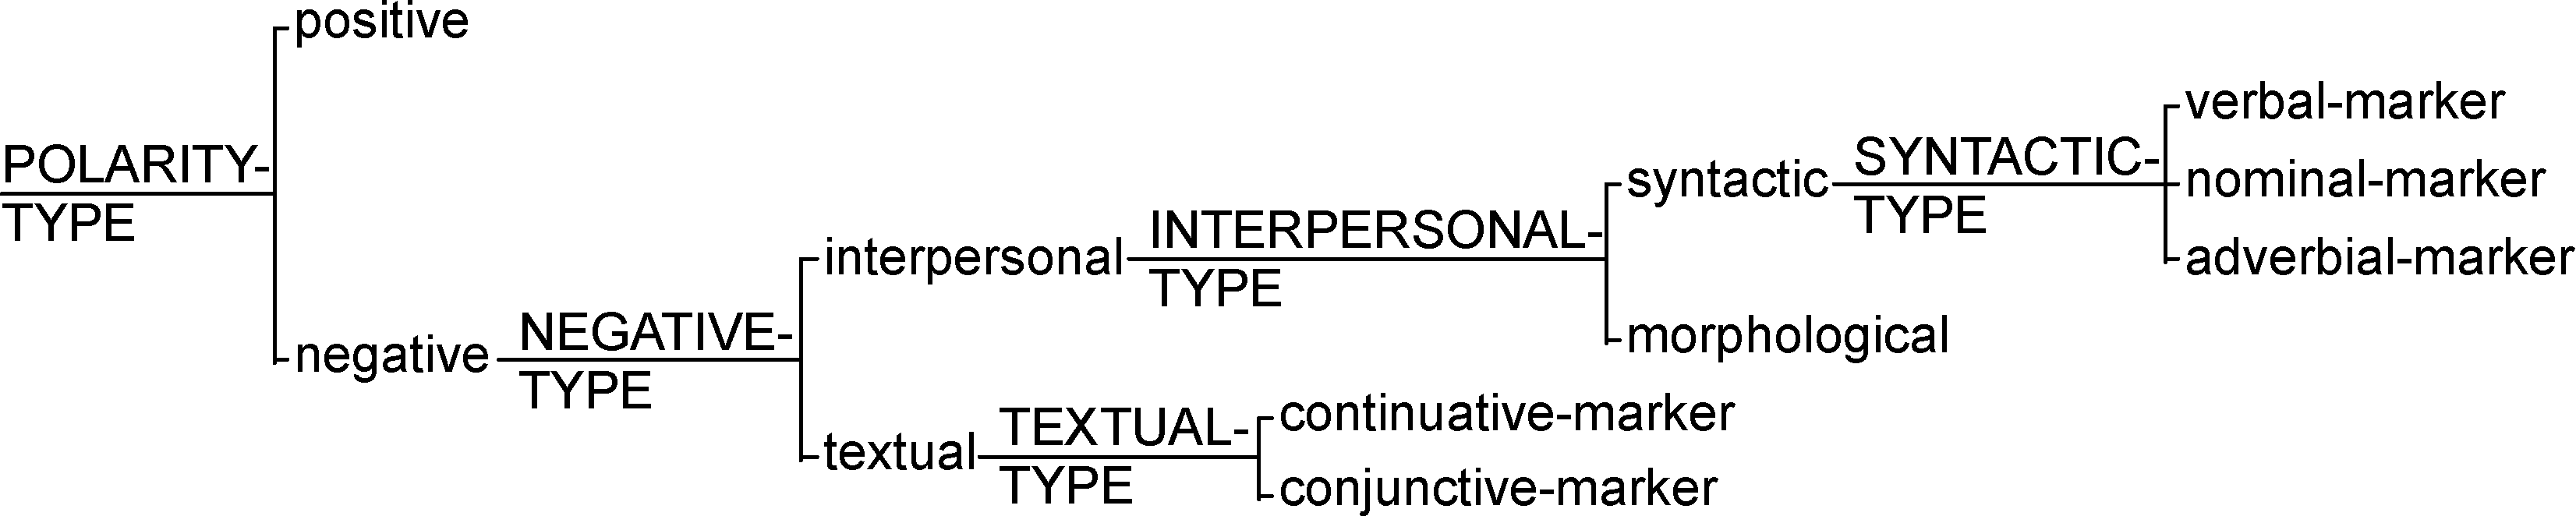
\includegraphics[width=\textwidth]{Figures/SFL-grammar/polarity-system.pdf}
	\caption{System network of POLARITY}
	\label{fig:polarity}
\end{figure}

In language it may be often the case that a choice in a system may lead to re-entering the same system again to make another choice again forming this way recursive systems. Alternatively, we can say that a system allows multiple choices for the same unit. These perspectives are the sides of the same coin where the recursion perspective is useful for natural language generation while multiple choice perspective suits better the parsing task and next I explain why by continuing the discussion on polarity system. 

The negative polarity in English clauses can be realised in several ways: via a noun group with intrinsic negative polarity feature like \textit{``nobody''} (\ref{ex:neg1}), negation particle of the verb \textit{``n't''} (\ref{ex:neg2}) or adverb with intrinsic negative polarity (\ref{ex:neg3}). 

\begin{exe}
	\ex\label{ex:neg1} Nobody with any sense is going. 
	\ex\label{ex:neg2} I don't have to mow my lawn.
	\ex\label{ex:neg3} Never expect her to come back.
\end{exe}

Consider now, the cases of double negation from the example \ref{ex:double-negatives1} where two kinds of negations are realised in the same clause: the negation by verb particle \textit{``n't''} and the pronoun \textit{``nobody''}. 

\begin{exe}
	\ex \label{ex:double-negatives1}
	Nobody with any sense isn't going. 
	\ex \label{ex:double-negatives2} I don’t have nobody to mow my lawn.
\end{exe}

The systems can be recursive and thus choices are not always mutually exclusive. Even though the system network  clearly distinguishes one type of negation from another multiple negations can still occurring simultaneously. Note that this more delicate distinctions in kind of negation, still is a negation and for any of them it is impossible to co-occur with positive polarity. 
The issue here is not semantic about whether the clause is positive or negative but what kinds of grammatical choices can be identified within the clause. The problem of whether the double negation shall be interpreted as positive is not necessarily as relevant as the task of identifying the two instances of negation. 

Halliday states that the speaker makes only one choice from a system. If this rule is interpreted as two choices from the same system at a time being impossible then it clearly does not cover the recursive systems and needs weakening to accommodate border cases. I propose relaxing the constraint of \textit{mutual exclusivity} to \textit{disjunction}. Correspondingly, two types of systemic networks emerge differing by \textit{the relation among choices}: the original Hallidayan XOR systems (such as POLARITY TYPE in figure \ref{fig:polarity}) and the OR systems for accommodating cases of multiple feature selections (such as SYSTEMIC TYPE in the same figure).

% entry condition relationship types
As system is expanded in delicacy to forms a systemic network of choices. Choice of a feature in one system becomes the entry condition for choices in more delicate systems below. I turn now to discuss the relationship types of relationships forming entry conditions to more delicate systems. For instance, an increase in delicacy can be seen as a taxonomic ``is a'' relationship between features of higher systems and lower systems like in the case of POLARITY TYPE and NEGATIVE TYPE in figure \ref{fig:polarity}. 

\begin{figure}[hbtp]
	\centering
	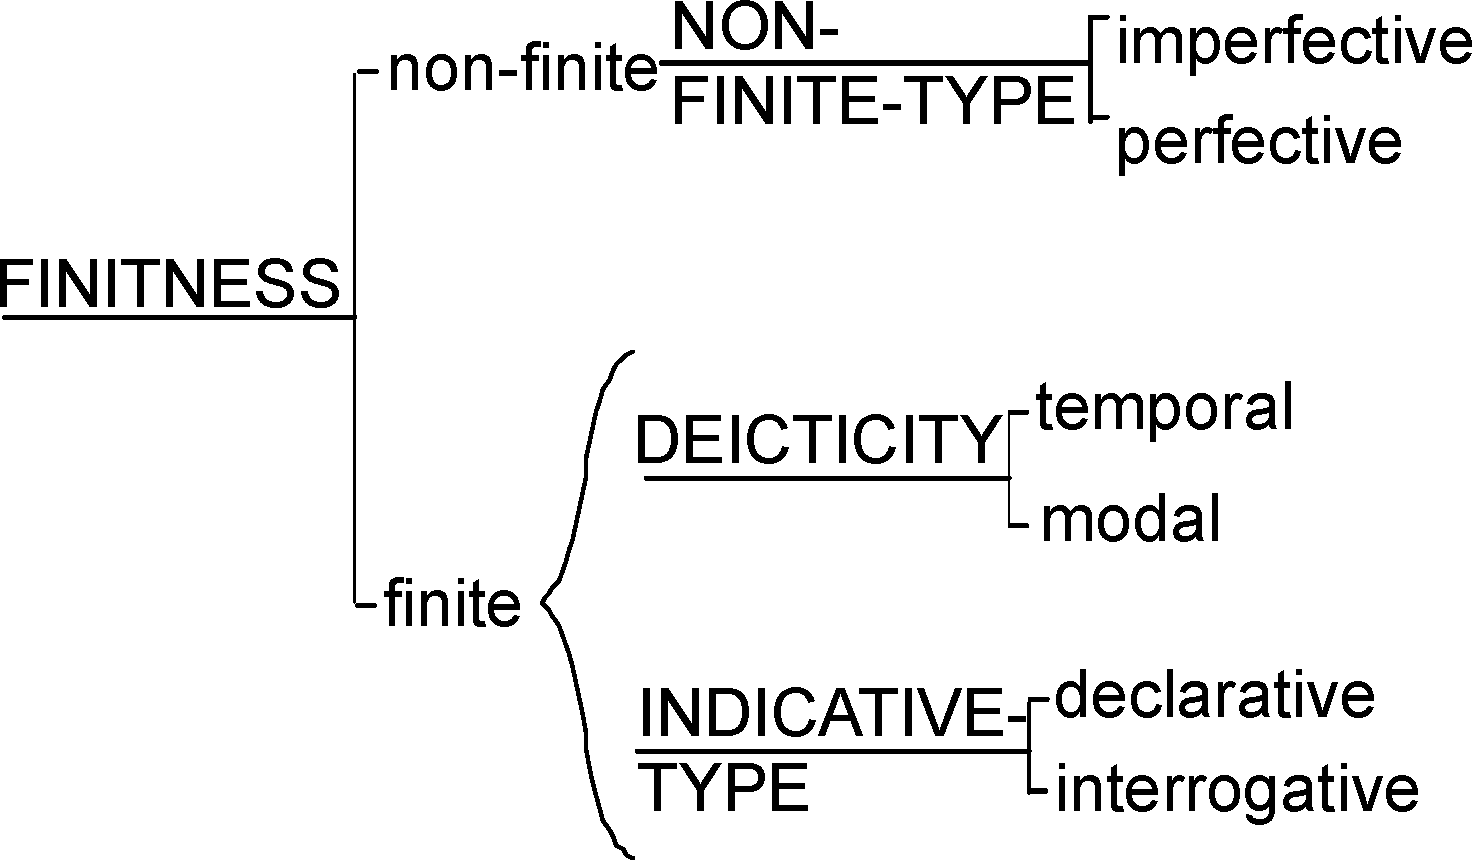
\includegraphics[width=0.5\textwidth]{Figures/SFL-grammar/finitness-system.pdf}
	\caption{A fraction of the finiteness system where increase of delicacy is not ``is a'' relation}
	\label{fig:finitness-fraction}
\end{figure}

The activation relation among systems in the cline of delicacy is not always taxonomic. Another relation is ``enables selection of'' without a any sub-categorisation implied. For example see FINITENESS system in figure \ref{fig:finitness-fraction} where in case that the finite option is selected then what this choice enables are not subtypes of finite but merely other options that become available i.e. DEIXIS and INDICATIVE TYPE. The latter is there because selection of finite implies also selection of indicative feature in a FINITNES's sibling system MOOD-TYPE comprised of options indicative vs. imperative. 

In this subsection I defined the system and systemic network, presented two system types by the relationship between their choices and distinguished two kinds of activation relations between systems on the cline of delicacy.

\subsection{coordination as unit complexing}
%TODO: the complex class is semantic and not grammatical
%TODO: sometimes the second element is more representative of the complex or the first one maybe, maybe just take the class of the first unit and then ingnore teh class of the rest, or the last one and ingnore classes of the first ones

\label{sec:coordination}
In SG unit complexes fill an important part of the grammar along with the \textit{taxis relations} which express the interdependency relations in unit complexes. \textit{Parataxis} relations bind units of equal status while the \textit{Hypotaxis} ones bind the dominant and  the dependant units. Fawcett bypasses the taxis relations replacing them with coordination and embedding \citep[p.~271]{Fawcett2000} seemingly an oversimplified approach leading to abandonment of unit complexing as well. While embedding accounts for the depth and complexity of syntax his approach to coordination is problematic. I further discuss and argue for utility of unit-complexes for the coordination but this idea can be further extended to other phenomena which involve fixed idiomatic structures such as comparatives or conditionals.

Coordination is challenge not only for SFL but for other linguistic theories as well. CG treats this phenomena as two or more units filling or expounding the same element. For example, in table \ref{ex:Cardiff-example-analisys} ``his shirt'' and ``and his jeans'' are two nominal groups that are siblings and both of them fill the same complement. 

\begin{table}[h]
	\centering
	\begin{tabular}{|c|c|c|c|c|c|c|}
		\hline
		\textit{Ike} & \textit{washed} & \textit{his} & \textit{shirt} & \textit{and} & \textit{his} & \textit{jeans} \\ \hline
		Subject         & Main Verb               & \multicolumn{5}{c|}{Complement}                                                    \\ \hline
		&                 & \multicolumn{2}{c|}{Nominal Group}      & \multicolumn{3}{c|}{Nominal Group}                     \\ \hline
		&                 & Deictic Determiner           & Head              & \&           & Deictic Determiner           & Head              \\ \hline
	\end{tabular}
	\caption{Coordination analysis in Cardiff Grammar}
	\label{ex:Cardiff-example-analisys}
\end{table}

In SG the coordination is analised as a \textit{complex unit} held together through paratactic relations ensuring that only one unit fills an element of the parent constituent in our example the complement of the clause. The table \ref{ex:Sydeny-example-analisys} illustrates an example analysis involving the complex unit approach. 

\begin{table}[h]
	\centering
	\begin{tabular}{|c|c|c|c|c|c|c|}
		\hline
		\textit{Ike}     & \textit{washed}      & \textit{his} & \textit{shirt} & \textit{and} & \textit{his} & \textit{jeans} \\ \hline
		Subject          & Predicate/Finite     & \multicolumn{5}{c|}{Complement}                                              \\ \hline
		\multicolumn{2}{|c|}{\multirow{3}{*}{}} & \multicolumn{5}{c|}{nominal group complex}                                   \\ \cline{3-7} 
		\multicolumn{2}{|c|}{}                  & \multicolumn{2}{c|}{1}        & \multicolumn{3}{c|}{+2}                      \\ \cline{3-7} 
		\multicolumn{2}{|c|}{}                  & Deictic      & Thing          & \&           & Deictic      & Thing          \\ \hline
	\end{tabular}
	\caption{Coordination analysis in Sydney Grammar}
	\label{ex:Sydeny-example-analisys}
\end{table}

The opinions are divided by whether to invite the notion of a complex unit to handle coordination or not. If we dismiss the unit complex then an element could be filled by more than one units and if we adopt it then the complexing relations need to be accounted along with unit class and what is its structure.

I would argue for adoption of such unit type for two reasons. First, only units are accounted for structure while the elements can only be filled by an unit. Allowing multiple units to fill an element requires accounting at least for order if not also for the relation between the units. The structure as it is described in theories of grammar by Halliday \citep{Halliday2002} and Fawcett \citep{Fawcett2000} is defined in the unit and not the element. A unit has a specific possible structure in terms of places of elements however if an element is filled by two units simultaneously it constitutes a violation of the above principle as the order of those units is not accounted for but it matters.
\begin{exe}
	\ex\label{ex:conj2-extra-marker1}
	(Both my wife and her friend) arrived late.  
	\ex\label{ex:conj2-extra-marker11} * (And her friend both my wife) arrived late.
	\ex\label{ex:conj2-extra-marker2}
	I want the front wall (either in blue or in green). 
	\ex\label{ex:conj2-extra-marker21}
	* I want the front wall (or in green either in blue). 
\end{exe}

If the order would not have mattered then we could say that the conjunctions from the example \ref{ex:conj2-extra-marker1} can be reformulated into \ref{ex:conj2-extra-marker11} and the one from \ref{ex:conj2-extra-marker2} into \ref{ex:conj2-extra-marker21}. But such reformulations are grammatically incorrect. Obviously the places do matter and they need to be described in the unit structure. 

Secondly, the lexical items that signal the conjunction are not a part of the conjuncted units. This is contrary to what is being described in Cardiff and Sydney grammars. Fawcett present the Linker elements (\&) which are filled by conjunctions as parts of virtually any unit class placed in the first position of the unit. Halliday omits to discuss in IFG \citep{Halliday2013} the place of Linkers but implicitly proposes the same as Fawcett through his examples of paratactic relations at various rank levels where the lexical items signalling conjunction are included in the units they precede.

For example in the ``or in green'' the presence of ``or'' signalls the presence at least of one more unit of the same nature and does not contribute to the meaning of the prepositional group but to the meaning outside the group requiring presence of a sibling. Even more, the lack of a sibling most of the time would constitute an ungrammatical formulation. I say sometimes because it is perfectly acceptable to start a clause/sentence with a conjunction most often ``but''. But even in those cases it still invites the presence of a sibling clause/sentence preceding the current one to be resolved at the discourse level. 

So conjunctions and pre-conjunctions shall not be placed as elements of the conjuncted units because they do not contribute to their meaning.

Adopting the unit complex and in particular coordination unit requires two clarifications (1) does the unit complex carry a syntactic class, and if so according to which criteria is it established? (2) Does it have any intrinsic features or not?

Zhang states in her thesis that the coordinating constructions do not have any categorial features thus there is no need to provide a new unit type. Instead the categorial properties of the conjuncts are transferred upwards \citep{NinaZhang2010}. For example if two nominal groups are conjuncted then the complex receives the nominal class. This principle holds for most of the cases however there are rare cases when the units are of different classes. Consider the example \ref{ex:conj3-different-unit-types} where the conjuncts are a nominal group ``last Monday'' and a prepositional group ``during the previous weekend''.
\begin{exe}
	\ex\label{ex:conj3-different-unit-types}
	I lost it (either last Monday or during the previous weekend). 
\end{exe}

%In unit types are of different classes: a nominal group and a prepositional phrase.
In this case there are two unit types that can be raised and it is not clear how to resolve this case. Options are to leave the class unspecified, transfer the class of the first unit upwards, or semantically resolve the class as both represent temporal circumstances even if they are realised through two different syntactic categories. Another option is to leave the class generic and assign the conjunction unit the class of \textit{``coordination complex''} without sub-classifying it according to the constituent units below, i.e. without upward unit class transfer. 

I address the second question regarding the intrinsic features of the complex unit. The coordination complex can have categorial features which none of the constituting units has. In the example \ref{ex:conj-plural-right} the conjunction of two singular noun groups requires plural agreement with the verb. Even though semantic interpretation that only one item is selected at a time, syntactically both items are listed in the clause and attempting third person singular verb forms like in \ref{ex:conj-plural-wrong} is grammatically incorrect.
\begin{exe}
	\ex\label{ex:conj-plural-right}
	A pencil or a pen \textbf{are} equally good as a smart-phone.
	%\ex\label{ex:conj-plural-right1} A fork and knife \textit{have} to be placed on the sides of each plate.
	\ex\label{ex:conj-plural-wrong} * A pencil or a pen \textbf{is} equally good as a smart-phone.
	%\ex\label{ex:conj-plural-wrong1} * A fork and knife \textit{has} to be placed on the sides of each plate.
\end{exe}
\begin{figure}[hbtp]
	\centering
	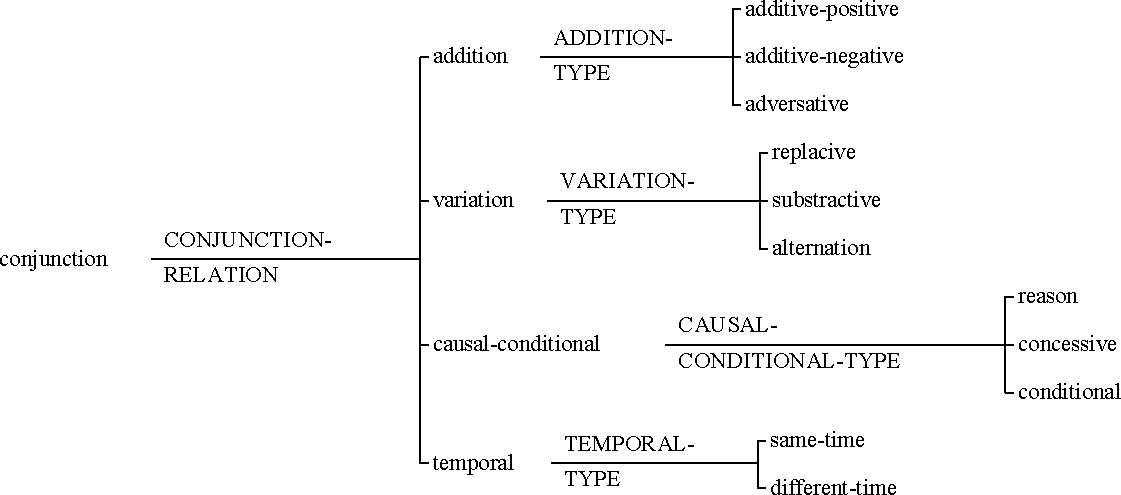
\includegraphics[width=\textwidth]{Figures/SFL-grammar/conjunction-system.pdf}
	\caption{Systemic network of coordination types}
	\label{fig:conj-rel-types}
\end{figure}

In the case of nominal group conjunction we can see that the plural feature emerges even if each individual unit is singular. For other unit classes it is not so obvious whether there are any linguistic features that emerge to the conjunction level. The meaning variation is rather semantic as for example conjunction of two verbs or clauses might mean very different things like consecutive actions, concomitant actions or presence of two states at the same time and so on. This brings us to another feature of the coordination complex - the type of the relationship it constructs. The lexical choice of head conjunct is the indicator of relationship among the conjuncts. Either \textit{and}, \textit{or}, \textit{but}, \textit{yet}, \textit{for}, \textit{nor} or \textit{so} they express different meanings which are well representable as a  relationship types systemic network in figure \ref{fig:conj-rel-types}.


%The coordination complex has a structure as depicted in figure \ref{fig:coord-complex-elements}. The lexical item signalling the coordination complex is the head of the construction. The Conjunct elements are the ones being related to each other and they can be filled or expounded by virtually any unit type. The Enumerator element substitutes the head and delimits the Conjuncts when there are more than two of them. The Enumerator is almost always a comma in written texts. 

Adopting the unit complexing enables various kinds of constructions and coordination is only one of them. Below we discuss taxis relations and their role in unit complexing.

\section{Critical discussion of the grammatical units}
\label{sec:discussion-unit-classes}

Now that the important theoretical details have been covered I would like focus on the grammars of the two schools. They have common parts and also differ in large parts on their paradigmatic and syntagmatic descriptions. This section discusses the main units considered in each of the grammars. Like in the previous section I argue on pragmatic grounds for adoption of unit structures from either grammar. This may seem like an inconsistency add below I try to convince you of the opposite below. The argument runs along the line that some unit structures are closer to the syntactic analysis and thus are easier to detect and parse and the other ones may be a level of abstraction higher falling more on the semantic grounds thus becoming more difficult to capture in structural variance and requiring lexico-semantic resources.

For the reasons of limited space I skipped introducing the Sydney and Cardiff grammars and in turn assume that the reader is familiar with the details fo both of them. And for a general overview of the unit structure in each of the grammars please refer to Appendix \ref{ch:syntax-overview}. Nevertheless, as it is a parallel contrastive discussion, even if the reader is familiar with one grammar only I hope it becomes clear how does certain phenomena are dealt with in the other one. 

\subsection{The verbal group and clause division}
\label{sec:verbal-grpoup-and-clause-division}
In SG the verbal group is described as an expansion of a verb just like the nominal group is the expansion of the noun\citep[p.396]{Halliday2013}. There are certainly words that are closely related and syntactically dependent on the verb all together forming a unit that functions as a whole. For example the auxiliary verbs, adverbs or the negation particles are words that are directly linked to a lexical verb. The verb group functions as Finite + Predicator elements of the clause in mood structure and as Process in Transitivity structure. 

In CG the verb group is dissolved moving the Main Verb as the pivotal element of the Clause unit. All the elements that form the clause structure and those that form the verb group structure are brought up together to the same level as elements of a clause. The clause structure in CG comprises elements with clause related functions(like Subject, Adjunct, Complement etc.) and other elements with Main Verb related functions(Auxiliary, Negation particle, Finite operator etc.).

Regarding from the Hallidayan rank scale perspective, merging the elements of the verb group into clause structure is not permitted because the units are of different rank scales. However it is not a problem for the relaxed rank scale version presented in subsection \ref{sec:rank-system}. The reason for adopting such an approach is best illustrated via complex verb groups with more than one non-auxiliary verb such as in examples \ref{ex:complex-verb-groups1}--\ref{ex:complex-verb-groups3}. 

Next I address the impact of this merger on (a) the clause structure (b) the clause boundaries and (c) semantic role distribution within the clause.

\begin{exe}
	\ex\label{ex:complex-verb-groups1}
	(The commission \textbf{started to investigate} two cases of overfishing in Norway.)  
	\ex\label{ex:complex-verb-groups2}
	(The commission \textbf{started} (\textbf{to investigate} two cases of overfishing in Norway.))
	\ex\label{ex:complex-verb-groups3}
	(The commission \textbf{started} (\textbf{to finish} (\textbf{investigating} two cases of overfishing in Norway.)))
\end{exe}

%Then answers to the above questions boil down to whether we allow for more than one lexical verb per predicate or not. 
In SG ``started to investigate'' (example \ref{ex:complex-verb-groups1}) is considered a single predicate of investigation which has specified the aspect of event incipiency despite the fact that there are two lexical verbs within the same verbal group. The ``starting'' doesn't constitute any kind of process in semantic terms but rather specifies aspectual information about the investigation process. The boundaries of the clause governed by this predicate stretch to entire sentence.

Semantically it is a sound approach because despite the presence of two lexical verbs there is only one event. However allowing such compositions leads to unwanted syntactic analysis for multiple lexical verb cases like in example \ref{ex:complex-verb-groups3}.To solve this kind of problems Fawcett dismisses the verb groups and merges their elements into clause structure. He proposes the syntactically elegant principle of \textit{``one main verb per clause''} \citep{Fawcett2008}. Apply this principle to the same sentence yields a structure of two clauses illustrated in example \ref{ex:complex-verb-groups2} where the main clause is governed by the verb ``to start'' and the embedded one by the verb ``to investigate''. Note the conflict between ``one main verb per clause'' with Halliday's principle that only whole units form the constituency of others (the (c) principle of rank scale described in subsection \ref{sec:rank-system}). So allowing incomplete groups into the constituency structure would breach entire idea of unit based constituency. 

Semantically the clause in SFL is a description of an event or situation as a figure with a process, participants and eventually circumstances where the process is realised through a lexical verb. Looking back to our examples, does the verb ``to start'' really describes a process or merely an aspect of it? Halliday treats such verbs as aspectual and when co-occurring with other lexical verbs are considered to form a single predicate. Accommodating Fawcett's stance, mentioned above and contradicting Halliday's approach, requires weakening the semantic requirement and allowing aspectual verbs to form clauses that contribute \textit{aspectually or modally} to the embedded ones. I mention also the modal contribution because some verbs like \textit{want, wish, hope}, etc. behave syntactically exactly like the aspectual ones. Moreover, Fawcett introduces into CG Transitivity network ``influential'' process type including all categories of meanings that semantically function as process modifiers: tentative, failing, starting, ending etc.

Fawcett's ``one main verb per clause'' principle changes the way clauses are partitioned, leads to abolition of the verbal group and introduces the ``influential'' process type.

\subsection{The Clause}
\label{sec:cardiff-clause}
It is commonly agreed in linguistic communities that the unit of clause is one of the core elements in human language. It is consider the syntactic unit that expresses semantic units of a situation referring to a potentially rich array of meanings. The clause structure has been studied for long time and the main clause constituents are roughly the same in SFL as the ones in the traditional grammar \citep{Quirk1985}, transformational grammar \citep{Chomsky1957} an indirectly in dependency grammar \citep{Hudson2010}.

In current work I adopt the CG Clause structure with the \textit{Main Verb} as pivotal element. Though there is no element that is obligatorily realised in English language, the Main Verb is realised with a reliably high degree of probability. Exceptions are the minor clauses (exclamations, calls, greetings and alarms) that occur in conversational contexts and elliptical clauses \citet{Halliday2013} such as the one in example \ref{ex:elipted-clause} which are not currently covered.

\begin{exe}
	\ex\label{ex:elipted-clause} They were in the bar, \textit{Dave in the restroom and Sarah by the bar}.
\end{exe}

As mentioned before \ref{structure} the elements of a structure are defined in terms of their function contributing to the formation of the whole unit. The elements of an English clause are \textit{Subject}, \textit{Finite}, \textit{Main Verb}(a part of the Predicator), up to two \textit{Complements} and a various number of \textit{Adjuncts}. All the elements of the assumed verbal group are part of the clause as well such as Auxiliary Verbs, Main Verb Extensions, Negators etc. (see Appendix \ref{ch:syntax-overview} for a complete list). 

%\todo*{}{TODO continue, maybe mention about the clause complexing}
%SFG accounts for how clauses form nexuses of tactic relations (see Definition \ref{def:taxis}).


\subsection{The Nominal Group}
\label{sec:nominal-group}
The nominal group expresses things, classes of things or a selection of instances in that class. In the table \ref{tab:example-ng} is presented an example analysis of the nominal group proposed in Sydney grammar \citep[pp.~364--369]{Halliday2013}. 
\begin{table}[!ht]
	\begin{tabular}{|c|c|c|c|c|c|}
		\hline
		\textit{those} & \textit{two} & \textit{old} & \textit{electric} & \textit{trains} & \textit{from Luxembourg} \\ \hline
		\multicolumn{4}{|c|}{pre-modifier}                               & head            & post-modifier            \\ \hline
		Deictic        & Numerative   & Epithet      & Classifier        & Thing           & Qualifyier               \\ \hline
		determiner     & numeral      & adjective    & adjective         & noun            & prepositional phrase     \\ \hline
	\end{tabular}
	\caption{The example of a nominal group in Sydeny Grammar}
	\label{tab:example-ng}
\end{table}

In SG it is constituted by a head nominal item modified by descriptors or selectors such as: \textit{Deictic}, \textit{Numerative}, \textit{Epithet}, \textit{Classifier}, \textit{Thing} and \textit{Qualifier}. Each element has a fairly stable correspondence to the word classes, expected to be expounded by lexical items. The table \ref{tab:function-pos-mapping} presents the mappings between the functions and the word classes.

\begin{table}[h]
	\begin{tabular}{|c|c|}
		\hline
		\textbf{Experiential function in noun group} & \textbf{class (of word or unit)} \\ \hline
		Deictic                             & determiner, predeterminer, pronoun \\ \hline
		Epithet                             & adjective                    \\ \hline
		Numerative                          & numeral(ordinal,cardinal)    \\ \hline
		Classifier                          & adjective, noun              \\ \hline
		Thing                               & noun                         \\ \hline
		Qualifier                           & prepositional phrase, clause \\ \hline
	\end{tabular}
	\caption{The mapping of noun group elements to classes}
	\label{tab:function-pos-mapping}
\end{table}

%There is little variation in how these functions are linked to the word classes. However the variation is not provided in the Sydney Grammar as it is in Cardiff Grammar. The latter provides data driven filling probabilities for each functional element to a set of possible unit classes \citep{Fawcett2000}.

The elements in CG differ from those of SG. The table \ref{tab:carfiff-ng} exemplifies a noun group analysed with CG covering all the possible elements. The table \ref{tab:cg-mappings} provides a legend for CG acronyms along with mappings to unit and word classes that can fill each element.

\begin{table}[H]
	\resizebox{\linewidth}{!}{
		\begin{tabular}{|c|c|c|c|c|c|c|c|c|c|c|c|c|c|c|}
			\hline
			\textit{or} & \textit{a photo} & \textit{of} & \textit{part} & \textit{of} & \textit{one} & \textit{of} & \textit{the best} & \textit{of} & \textit{the} & \textit{fine} & \textit{new} & \textit{taxis} & \textit{in Kew} & \textit{,} \\ \hline
			\multicolumn{12}{|c|}{pre-modifiers} & head & \multicolumn{2}{c|}{post-modifiers} \\ \hline
			\& & rd & v & pd & v & qd & v & sd or od & v & dd & m & m & h & q & e \\ \hline
		\end{tabular}}
		\caption{The example of a nominal group in Cardiff Grammar}
		\label{tab:carfiff-ng}
	\end{table}
	%
	\begin{table}[h]
		\begin{tabular}{|c|c|c|}
			\hline
			\textbf{symbol} & \textbf{function meaning} & \textbf{class (of word or unit)} \\ \hline
			rd & representational determiner & noun, noun group \\ \hline
			v & selector ``of'' & preposition \\ \hline
			pd & partitive determiner & noun, noun group \\ \hline
			fd & fractional determiner & noun, noun group, quantity group \\ \hline
			qd & quantifying determiner & noun, noun group, quantity group \\ \hline
			sd & superlative determiner & noun, noun group, quality group, quantity group \\ \hline
			od & ordinative determiner & noun, noun group, quality group \\ \hline
			td & tipic determiner & noun, noun group \\ \hline
			dd & deictic determiner & determiner, pronoun, genitive cluster \\ \hline
			m & modifier & adjective, noun, quality group, genitive cluster \\ \hline
			h & head & noun, genitive cluster \\ \hline
			q & qualifier & prepositional phrase, clause \\ \hline
			\& & linker & conjunction \\ \hline
			e & ender & punctuation mark \\ \hline
		\end{tabular}
		\caption{The mapping of noun group elements to classes in Cardiff grammar}
		\label{tab:cg-mappings}
	\end{table}
	%
	
	The elements in CG have are based on semantic criteria supported by lexical and syntactic choices. Consequently some elements cannot be derived based on solely syntactic criteria requiring semantically motivated lexical resources. Semantically bound elements are predominantly determiners \textit{Representational, Partitive, Fractional, Superlative, Typic Determiners} while the rest of the elements: \textit{Head, Qualifier, Selector, Modifier and Deictic, Ordinative and Quantifying Determiners} can be determined solely on the syntactic criteria. The latter correspond fairly well to Sydney version of nominal group which is adopted in present work with the  benefits of relaxed rank system replacing the sub-structures with embedded units and simplifying the syntactic structures. 
	
	%3. introduction of negation element, linker, punctuation
	%``No'' as determiner. negative pronoun noone.
	%\citep[p.~62,109,185]{Quirk1985}, \citep[p.~365--374]{Halliday2013}, 
	%
	%The negation element is in Cardiff Grammar in clause structure so that it is separated from the finite. It's adoption in noun structure might or might not be a good idea. It is useful for complex groups. 
	%
	%\begin{exe}
	%\ex \label{ex:example-of-no}
	%No breathing man or animal can escape that forest alive.
	%\end{exe} 
	
	Another simplification is renouncing to distinction between the Head and Thing \citep[p.~390--396]{Halliday2013} for the semantic ambiguity reasons as the determiners in CG. Thus if the logical Head of the nominal group is a noun then it is labelled as the Thing leaving the semantic discernment as a secondary process and out of the current scope. Otherwise, in cases of nominal groups without the Thing element, if the Head is pronoun(other than personal), numeral or adjective (mainly superlatives) then they function as Deictic, Numerative or Epithet. So I propose to parse the nominal groups in two steps: first determine the main constituting chunks and assign functions to the unambiguous ones and second perform a semantically driven evaluation for the less certain units.
	
%	\todo*{probably remove: discussion of Head/Thing and CG determiners distinction}{
		In other cases the Thing is present but it is different from the Head. Consider example \ref{ex:dectic-ngs}. In Sydney grammar they're treated as a nominal groups with qualifiers introduced by the \textit{``of''} preposition. But these nominal groups are not really about the ``cup'', ``some'' or ``another one'' but rather about ``tea'', ``youngsters'' and ``eruptions''. 
		\begin{exe}
			\ex \label{ex:dectic-ngs} (a cup) of (tea)
			\ex (some) of (those youngsters)
			\ex (another one) of (those periodic eruptions)
		\end{exe}
		So then the syntactic Head still remains the first noun in the nominal group, but then by a semantic evaluation the Thing is shifted into the Qualifier introduced by ``of'' preposition. Cardiff Grammar weakens the assumption that every prepositional phrase acts as Qualifier in a nominal group and it the special case of the preposition ``of''. It is allowed to act not as the element introducing a prepositional phrase but as a end mark of a determiner-like selector. Thus making the former noun group a determiner in the latter one. This approach shifts the noun group head into the position of semantically based Thing and erases the discrepancy problem between them. Nonetheless this is not straight forward solution as it requires lexical-semantic informed decision.
        % However this is not straight forward solution. There is a lot of space for variations the syntactic structure. 
        For example in \ref{ex:of-qualifiers} (Head/Thing marked in bold) the preposition ``of'' introduces Qualifiers. 
		\begin{exe}
			\ex \label{ex:of-qualifiers}
			He was the \textbf{confidant} of the prime minister.
			\ex It was the \textbf{clash} of two cultures.
		\end{exe}
		
		The distinction between cases when the proposition ``of'' introduces a Qualifier or ends a Selector/Deictic requires a semantic evaluation answering the questions ``what is the Thing that this nominal group is about?''. While it is easy to just assume that the first noun in the nominal group is the head. 
        
        Therefore, I propose to parse the nominal groups in two steps: first determine the main constituting chunks and assign functions to the unambiguous ones and then in the second step to perform a semantically driven evaluation for the less certain units. This evaluation can be performed by further capturing the structure of nominal groups that act as Dyslectics through their lexico-syntactic realisation patterns.
%	}
	
	\subsection{The Adjectival and Adverbial Groups}
	\label{sec:advectival-adverbial-groups}
%	\todo{Revise the whole subsection}
	Following the rationale of head-modifier like in the case of nominal groups, the adjectives and adverbs function as pivotal elements to form groups. The structure of adverbial and adjectival constructions is briefly covered in Sydney grammar in terms of head-modifier logical structures without an elaborated experiential structure like in the case of nominal groups. While the adverbial group is recognised as a distinct syntactic unit the adjectival group is treated as a special case of nominal group specifically as a sub-structure of Epithet or Classifier elements.
	
	\begin{exe}
		\ex\label{ex:lucky} He is \textit{very lucky}.
	\end{exe}
	
	For example ``very lucky'' in \ref{ex:lucky} is analysed as a short form of the nominal group ``very lucky one'' where ``lucky'' is the head of the nominal group with a missing Thing element ``one''. In this example ``very'' is not nominal modifier, it does not modify the missing nominal head but the adjective ``lucky'' so they constitute a head-modifier structure filling the Epithet element and as the rank scale system does not allow groups to fill elements of groups then it is described as a substructure of the nominal group.
	
	In SG ``The adverbial group has an adverb as Head which may or may not be accompanied by modifying elements''\citep[p.~419]{Halliday2013}. The adverbial groups may fill modal and circumstantial adjunct elements in a clause corresponding to eight semantic classes of: time, place, four types of manner and two types of assessment. The adverbial pre-modifiers express polarity, comparison and intensification along with only one comparison post-modifier \citep[p.420-421]{Halliday2013}. 
	
	
	A thorough systemic functional examination has been provided for the first time by Tucker \citet{Tucker1997,Tucker1998} materialised into a lexical-grammatical systematization of adjectives and the structure of Quality Group in CG. Fawcett uses the quality group structure for Adverbials as well as they follow similar grammatical behaviour. He avoids calling the group according to the word class but rather refers to the semantic meaning of what both groups express, i.e. the quality of things, situations or qualities themselves. The qualities of things have adjectives as their head while the qualities of situations an adverb. 
	
	In Cardiff Grammar, the head of the quality group is called \textit{Apex} while the set of modifying elements: \textit{Quality Group Deictic, Quality Group Quantifier, Emphasizing Temperer, Degree Temperer, Adjunctival Temperer, Scope} and \textit{Finisher}. The quality group most frequently fills complements and adjuncts in clauses and fill modifiers and superlative determiners in nominal groups but there are also other cases found in the data. 
	
	Just like in the case of nominal group the adverbial and adjectival groups in Cardiff grammar are semantically motivated. To automatically identify elements of the quality group requires lexico-semantic resources.
    
    Some adverbs are different from others at least because not all of them can be heads of the adverbial group like for example \textit{very, much, less, pretty} also being able to act as adjectival modifiers whereas others cannot. So a naive attempt is to use a list of words to identify the Emphasizing and Degree Temperers. 
    
    Other elements of the quality group like the \textit{Scoper} or \textit{Finisher} are more difficult to identify and localize as part of the group only by syntactic cues and/or lists of words because of their inherent semantic nature. The problem is similar to detecting whether a prepositional phrase is filling a qualifier element in the preceding nominal group or it is filling a complement or adjunct in the clause. Not surprisingly the Scopers and Finishers are most of the time prepositional phrases. 
	
	Another issue is continuity. The question is whether a grammar shall allow at least at syntactic level for discontinuous constituents or not. And then if so how to detect all the parts of the group even if they do not stand in proximity of each other. For example, comparatives, a complex case of a quality group, could be realised in a continuous or discontinuous forms. Compare the analyses presented in \ref{tab:csgq1} and \ref{tab:csgq2}. In the first case the comparative structure is a continuous quality group. In the second case the comparative is dissociated and analysed as separate adjuncts. 
	
	On one hand it is not a problem treating them as two adjuncts, because that is what they are from the syntactic point of view. However, semantically as Fawcett proposes, there is only one quality group with a discontinuous realisation whose Scope element is placed in a thematic position before the subject. 
	%
	\begin{table}[h]
		\centering
		\begin{tabular}{|c|c|c|c|l|c|c|}
			\hline
			\textit{I} & \textit{am} & \textit{much} & \textit{smarter} & \textit{today} & \textit{than} & \textit{yesterday} \\ \hline
			Subject & Main Verb & \multicolumn{5}{c|}{Adjunct} \\ \hline
			pronoun & verb & \multicolumn{5}{c|}{quality group} \\ \hline
			&  & Emphasizing Temperer & Apex & Scope & \multicolumn{2}{c|}{Finisher} \\ \hline
		\end{tabular}
		\caption{Comparative structure as one quality group adjunct}
		\label{tab:csgq1}
	\end{table}
	%
	\begin{table}[h]
		\centering
		\begin{tabular}{|c|c|c|c|c|c|c|}
			\hline
			\textit{Today} & \textit{I} & \textit{am} & \textit{much} & \textit{smarter} & \textit{than} & \textit{yesterday} \\ \hline
			Adjunct & Subject & Main Verb & \multicolumn{4}{c|}{Adjunct} \\ \hline
			adverb & pronoun & verb & \multicolumn{4}{c|}{quality group} \\ \hline
			&  &  & Emphasizing Temperer & Apex & \multicolumn{2}{c|}{Finisher} \\ \hline
		\end{tabular}
		\caption{Comparative structure split among two adjuncts}
		\label{tab:csgq2}
	\end{table}
	%
	For an automatic process to identify a complex quality group is a difficult task. It needs to pick up queues like a comparative form of the adjective followed by the preposition ``than'' and then look for two terms being compared. Given some initial syntactic structure such patterns could be modelled and applied but only as a secondary semantically oriented process.
	
	Since both the adverbial and adjectival groups have similar structures, it is syntactically feasible to automatically analyse them in terms of head-modifier structures in a first phase followed by a complementary process which assigns functional roles to the quality group components. 

\section{Discussion}

    This chapter introduces the fundamentals of systemic functional linguistics and presents an adaptation of Sydney and Cardiff theories of grammar to the task of parsing.
    
    Because of bottom up approach to unit structure, rank scale relaxation and accommodation of embedding as a general principle Cardiff systemic functional theory is more suitable for parsing than Sydney one. Nonetheless the unit definitions in Cardiff grammar are deeply semantic in nature. Parsing with such units requires most of the time lexical-semantic informed decisions beyond merely syntactic variations. This is one of the reasons why the parsing attempts by \citet{ODonoghue1991a} and others in COMMUNAL project were all based on a corpus.
    
    As there was no corpus available and because the parsing approach is based on syntactic backbone none of the theories could be fully used as such. The second part of the chapter attempts to merge and adapt the grammars and theories of grammar to this parsing approach.
    
    Next chapter lays the theoretical foundations of Dependency Grammar and introduces the Stanford dependency parser used as a departing point in current parsing pipeline. Because there is a transformation step from dependency to systemic functional consistency structure, next chapter also covers a theoretical compatibility analysis and how such a transformation should in principle look like. 

